\documentclass[a4paper,12pt]{report}

% --- Packages ---
\usepackage[utf8]{inputenc}
\usepackage[T1]{fontenc}
\usepackage[english]{babel}
\usepackage{geometry}
\geometry{top=3cm, bottom=3cm, left=3cm, right=3cm}
\setlength{\emergencystretch}{3em}
\usepackage{graphicx}
\usepackage{xcolor}
\usepackage{amsmath}
\usepackage{fancyhdr}
\usepackage{float}
\usepackage{booktabs}
\usepackage{enumitem}
\usepackage{listings}
\usepackage{bibentry}
\usepackage{csquotes}
\usepackage[dvipsnames]{xcolor}
\usepackage{natbib}
\usepackage[hidelinks]{hyperref}

% --- FONT: Roboto (Modern Sans-Serif) ---
\usepackage[sfdefault]{roboto}

% --- Custom Colors ---
\definecolor{PhaseBlue}{RGB}{73, 96, 209}
\definecolor{PhaseGray}{RGB}{85, 85, 85}
\definecolor{PhaseMagenta}{RGB}{189, 41, 107}

% --- HEADING STYLING ---
\usepackage{titlesec}

% 1. PART Styling (e.g., "Module 1") -> PHASE BLUE
\titleformat{\part}[display]
  {\bfseries\fontsize{60}{50}\selectfont\color{PhaseBlue}\centering} % Format
  {}
  {20pt}                % Spacing
  {\Huge}               % Title size

% 2. CHAPTER Styling (e.g., "Automated SAR...") -> PHASE MAGENTA
\titleformat{\chapter}[display]
  {\bfseries\Huge\color{PhaseMagenta}} % Format: Bold, Huge, Magenta
  {\filleft\fontsize{60}{60}\selectfont\color{PhaseMagenta!30}\thechapter} % Number: Giant, faded magenta, right
  {1ex}
  {\titlerule[2pt]\vspace{1.5ex}\filleft} % Line: Thick, aligned right
  [\vspace{1ex}]

% 3. SECTION Styling (Standard Black/Dark Grey)
\titleformat{\section}
  {\Large\bfseries\color{black}}
  {\thesection}{1em}{}

% --- Header/Footer Setup ---
\pagestyle{fancy}
\setlength{\headheight}{15pt}
\fancyhf{}
\fancyhead[L]{\textcolor{PhaseGray}{\small PHASE Manual}}
\fancyhead[R]{\textcolor{PhaseGray}{\small \leftmark}}
\fancyfoot[C]{\thepage}
\renewcommand{\headrulewidth}{0.4pt}
\definecolor{PhaseGray}{RGB}{100, 100, 100}

\begin{document}
\nobibliography*

% --- TITLE PAGE ---
\begin{titlepage}
    \centering
    \vspace*{1cm} % Adjusted spacing

    % Logo
    
\includegraphics[width=0.8\textwidth]{images/PHASE_logo.png}

    \vspace{4cm}

    %\noindent\makebox[\linewidth]{\rule{\textwidth}{1pt}} \\[0.5cm]

    {\fontsize{40}{48}\selectfont \textbf{USER MANUAL}}\\[0.5cm]
    {\Large \textcolor{PhaseGray}{Version 7.0.0}}

    \vspace{3cm}

    % Icons
    
\includegraphics[width=0.8\textwidth]{images/Icons.png}

    \vfill

    \textbf{\large Authors}\\[0.2cm]
    \large Roberto Monti, Lorenzo Rossi, Mirko Reguzzoni\\[0.2cm]
    \textit{\color{PhaseBlue}\large Politecnico di Milano}\\[1cm]

    {\small Last update: \today}
\end{titlepage}

\pagenumbering{roman}
\tableofcontents
\clearpage
\pagenumbering{arabic}

% --- Content Starts Here ---

\chapter{Introduction}

PHASE (Persistent Scatterer Highly Automated Suite for Environmental Monitoring) is an end-to-end application for SAR preprocessing, Persistent Scatterer Interferometry (PSI), and displacement modeling. Version 7 brings the three stages into one hub: \textbf{Preprocessing}, \textbf{StaMPS PSI}, and \textbf{Displacement Modeling}. The pipeline supports Sentinel-1 and COSMO-SkyMed (CSK/CSG) products and guides the user from SAR scenes to line-of-sight (LOS) displacement time series and modeled products. PHASE automates many operations but does not replace scientific quality control or independent validation.

\begin{figure}[htbp]
        \centering
        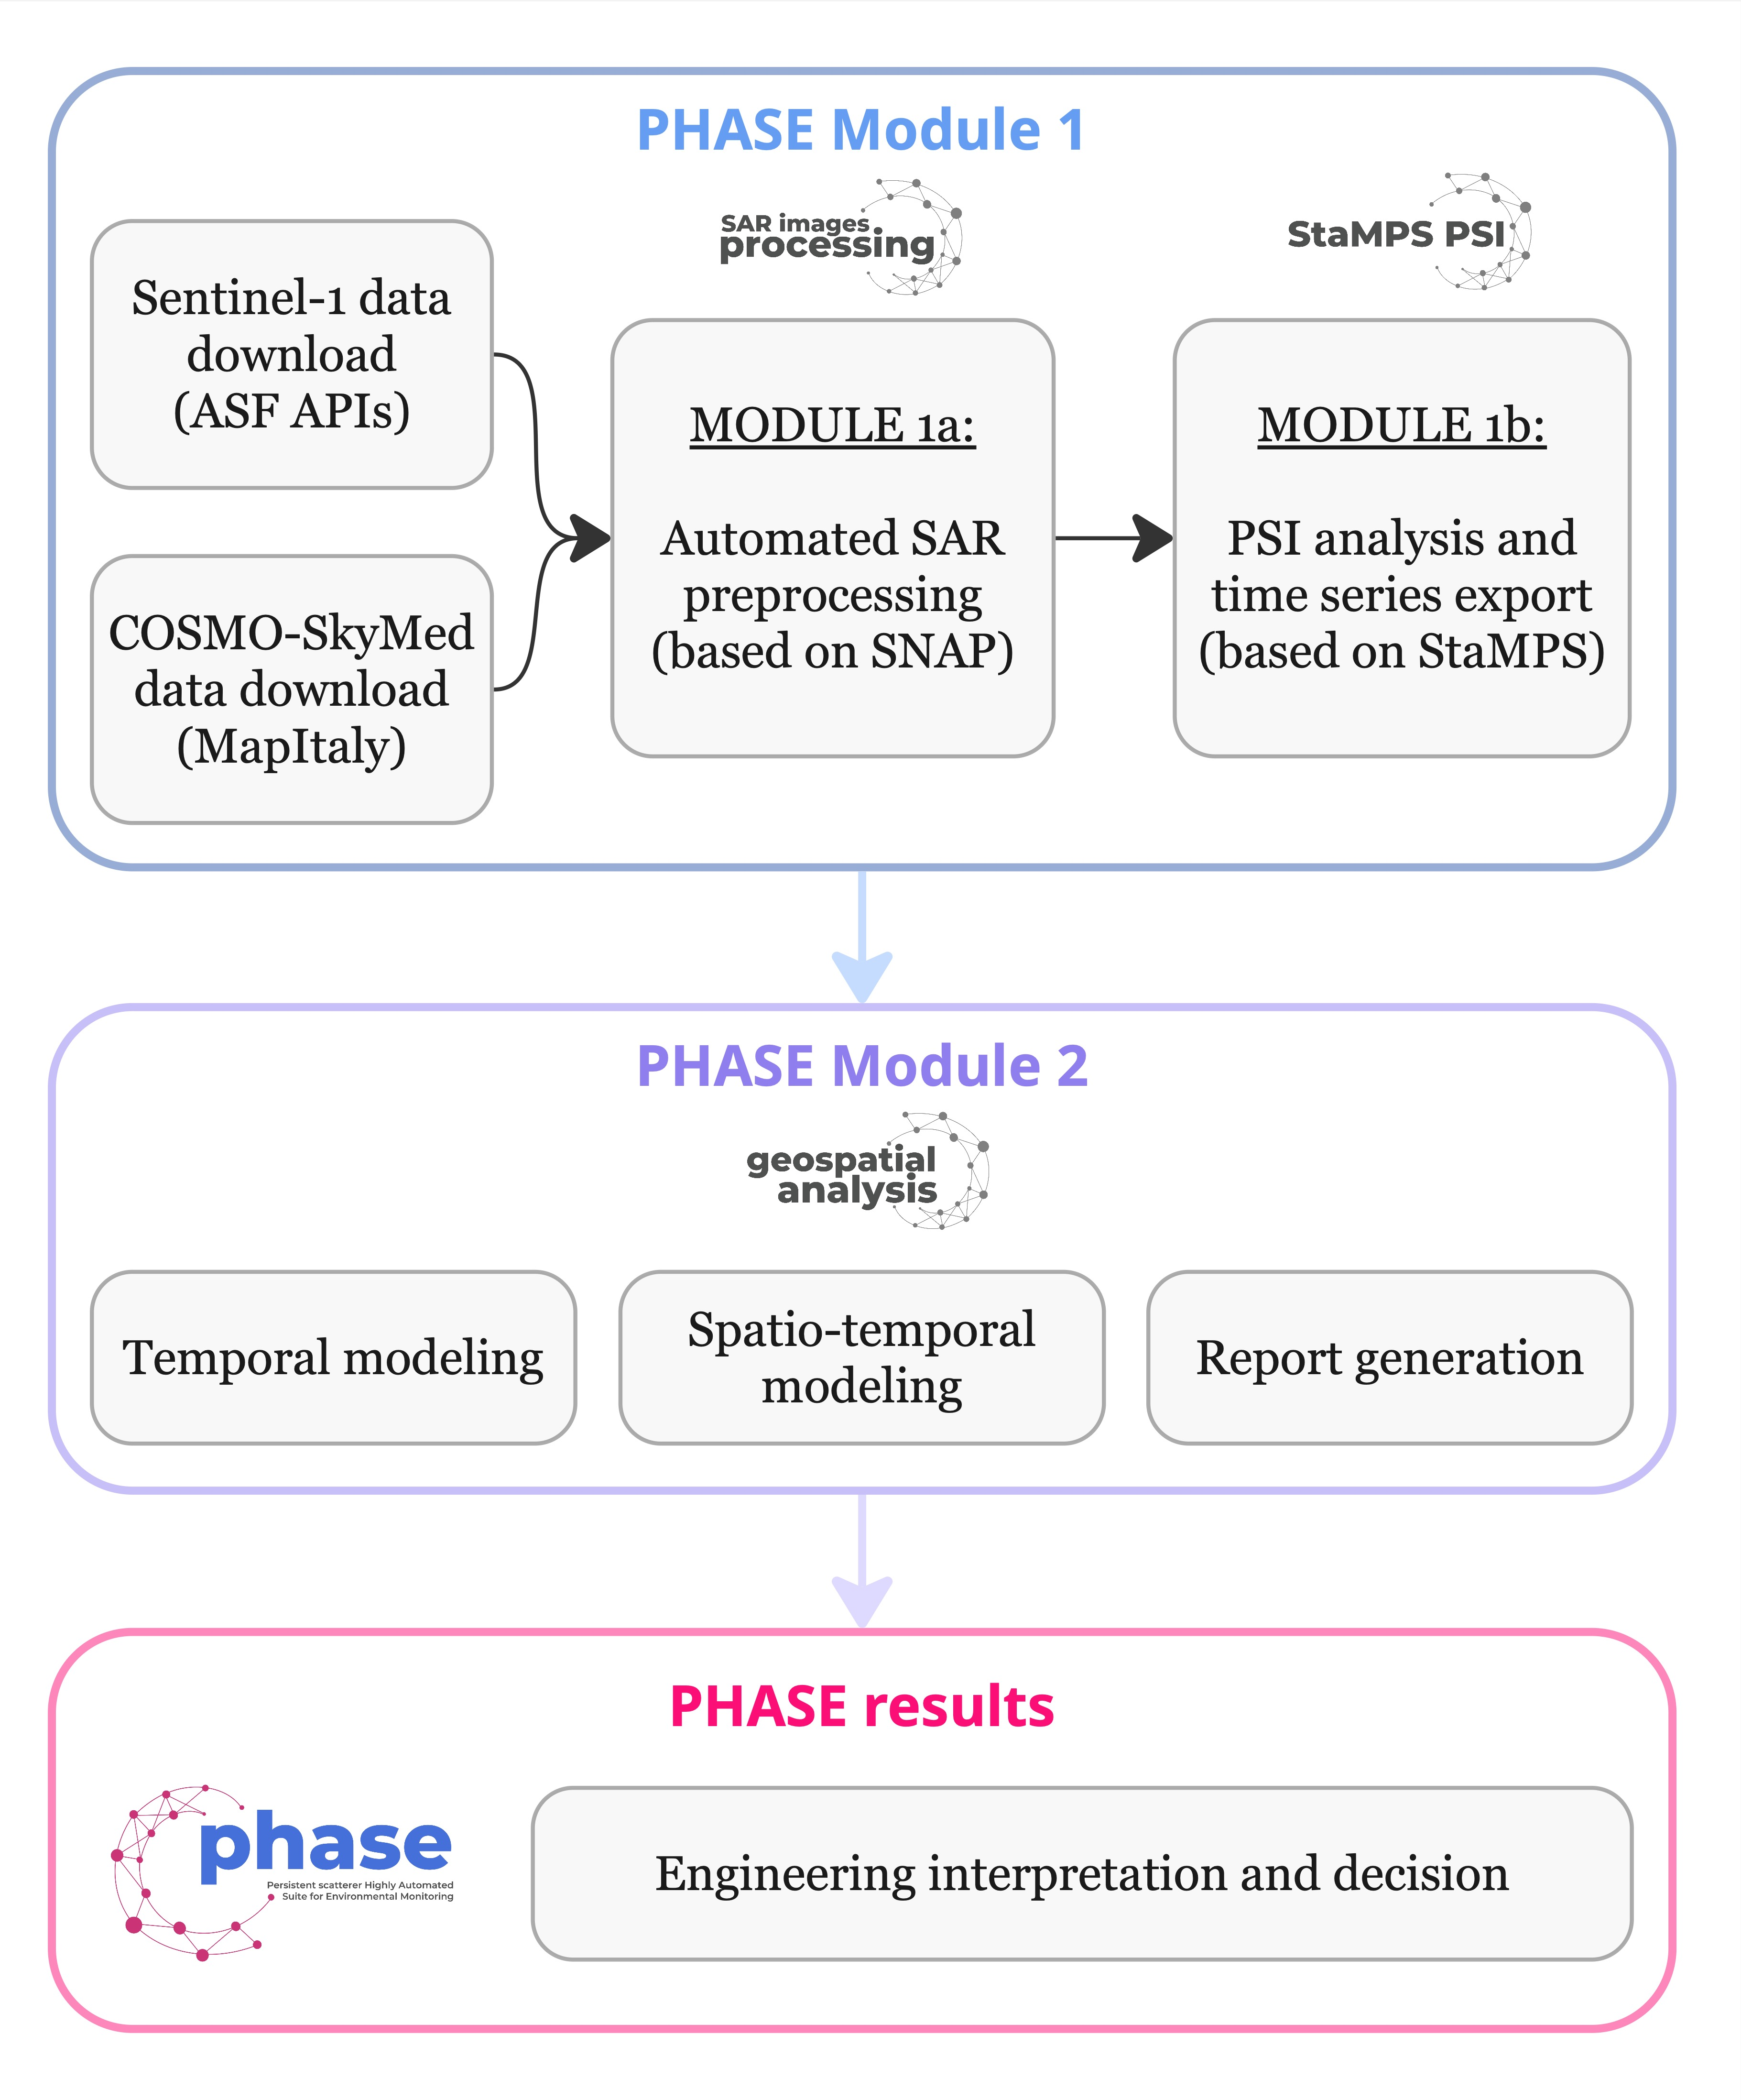
\includegraphics[width=1\textwidth]{images/PHASE_workf1.jpg}
        \caption{Conceptual PHASE workflow. The three stages are accessed from one application in version 7.}
\end{figure}

\subsection*{What changed in version 7}
PHASE is installed \emph{once per computer}; a project contains data and outputs, not another copy of the application. The hub keeps the same project open across all three modules, shows stage status, and provides a \textbf{Check for updates} control. The Preprocessing and StaMPS run monitors display progress and diagnostics. The optional TS Points picker is integrated into StaMPS PSI; complete time-series exports are produced automatically. PSI exports now offer an explicit standard/corrected choice, documented in Chapter 3.

\vspace{\baselineskip}
\noindent This manual covers the version 7 user workflow and the principal scientific choices. Consult the original SNAP, StaMPS and TRAIN documentation for full algorithmic details and parameter definitions.

\vspace{\baselineskip}
\section{Installation, projects and updates}
Download the installer for your system from \url{https://github.com/robimonti/PHASE/releases}. Use the release asset, not GitHub's \emph{Code--Download ZIP}. MATLAB and ESA SNAP are external prerequisites; follow the installer's checks and the current release notes for the supported versions and remaining dependencies.

\begin{itemize}
    \item \textbf{Windows 10/11:} run \texttt{install-phase.exe}. The guided installer and end-to-end workflow have been tested.
    \item \textbf{macOS Apple Silicon:} open the PHASE DMG and install PHASE. The preprocessing and StaMPS PSI pipelines, including Step 8 and TRAIN \texttt{a\_linear}, have been tested. Apple Intel is outside this release's supported scope. The app is not Developer-ID signed or notarized. If Gatekeeper blocks it, verify that the DMG came from the official release, attempt to open it, then use \emph{System Settings $\rightarrow$ Privacy \& Security $\rightarrow$ Open Anyway}. Do not disable Gatekeeper globally.
    \item \textbf{Linux x86\_64:} the AppImage/native build path is experimental. An end-to-end PSI run has not yet been validated on Linux. Consult the release notes and installer requirements before relying on it for research.
\end{itemize}

The app is installed only once. Launch \textbf{PHASE}, then select \textbf{New project} or \textbf{Open project}. Project folders may reside wherever you have sufficient space and write permission. Do not copy the PHASE engine or individual \texttt{.mlapp} files into each project.

\begin{figure}[htbp]
    \centering
    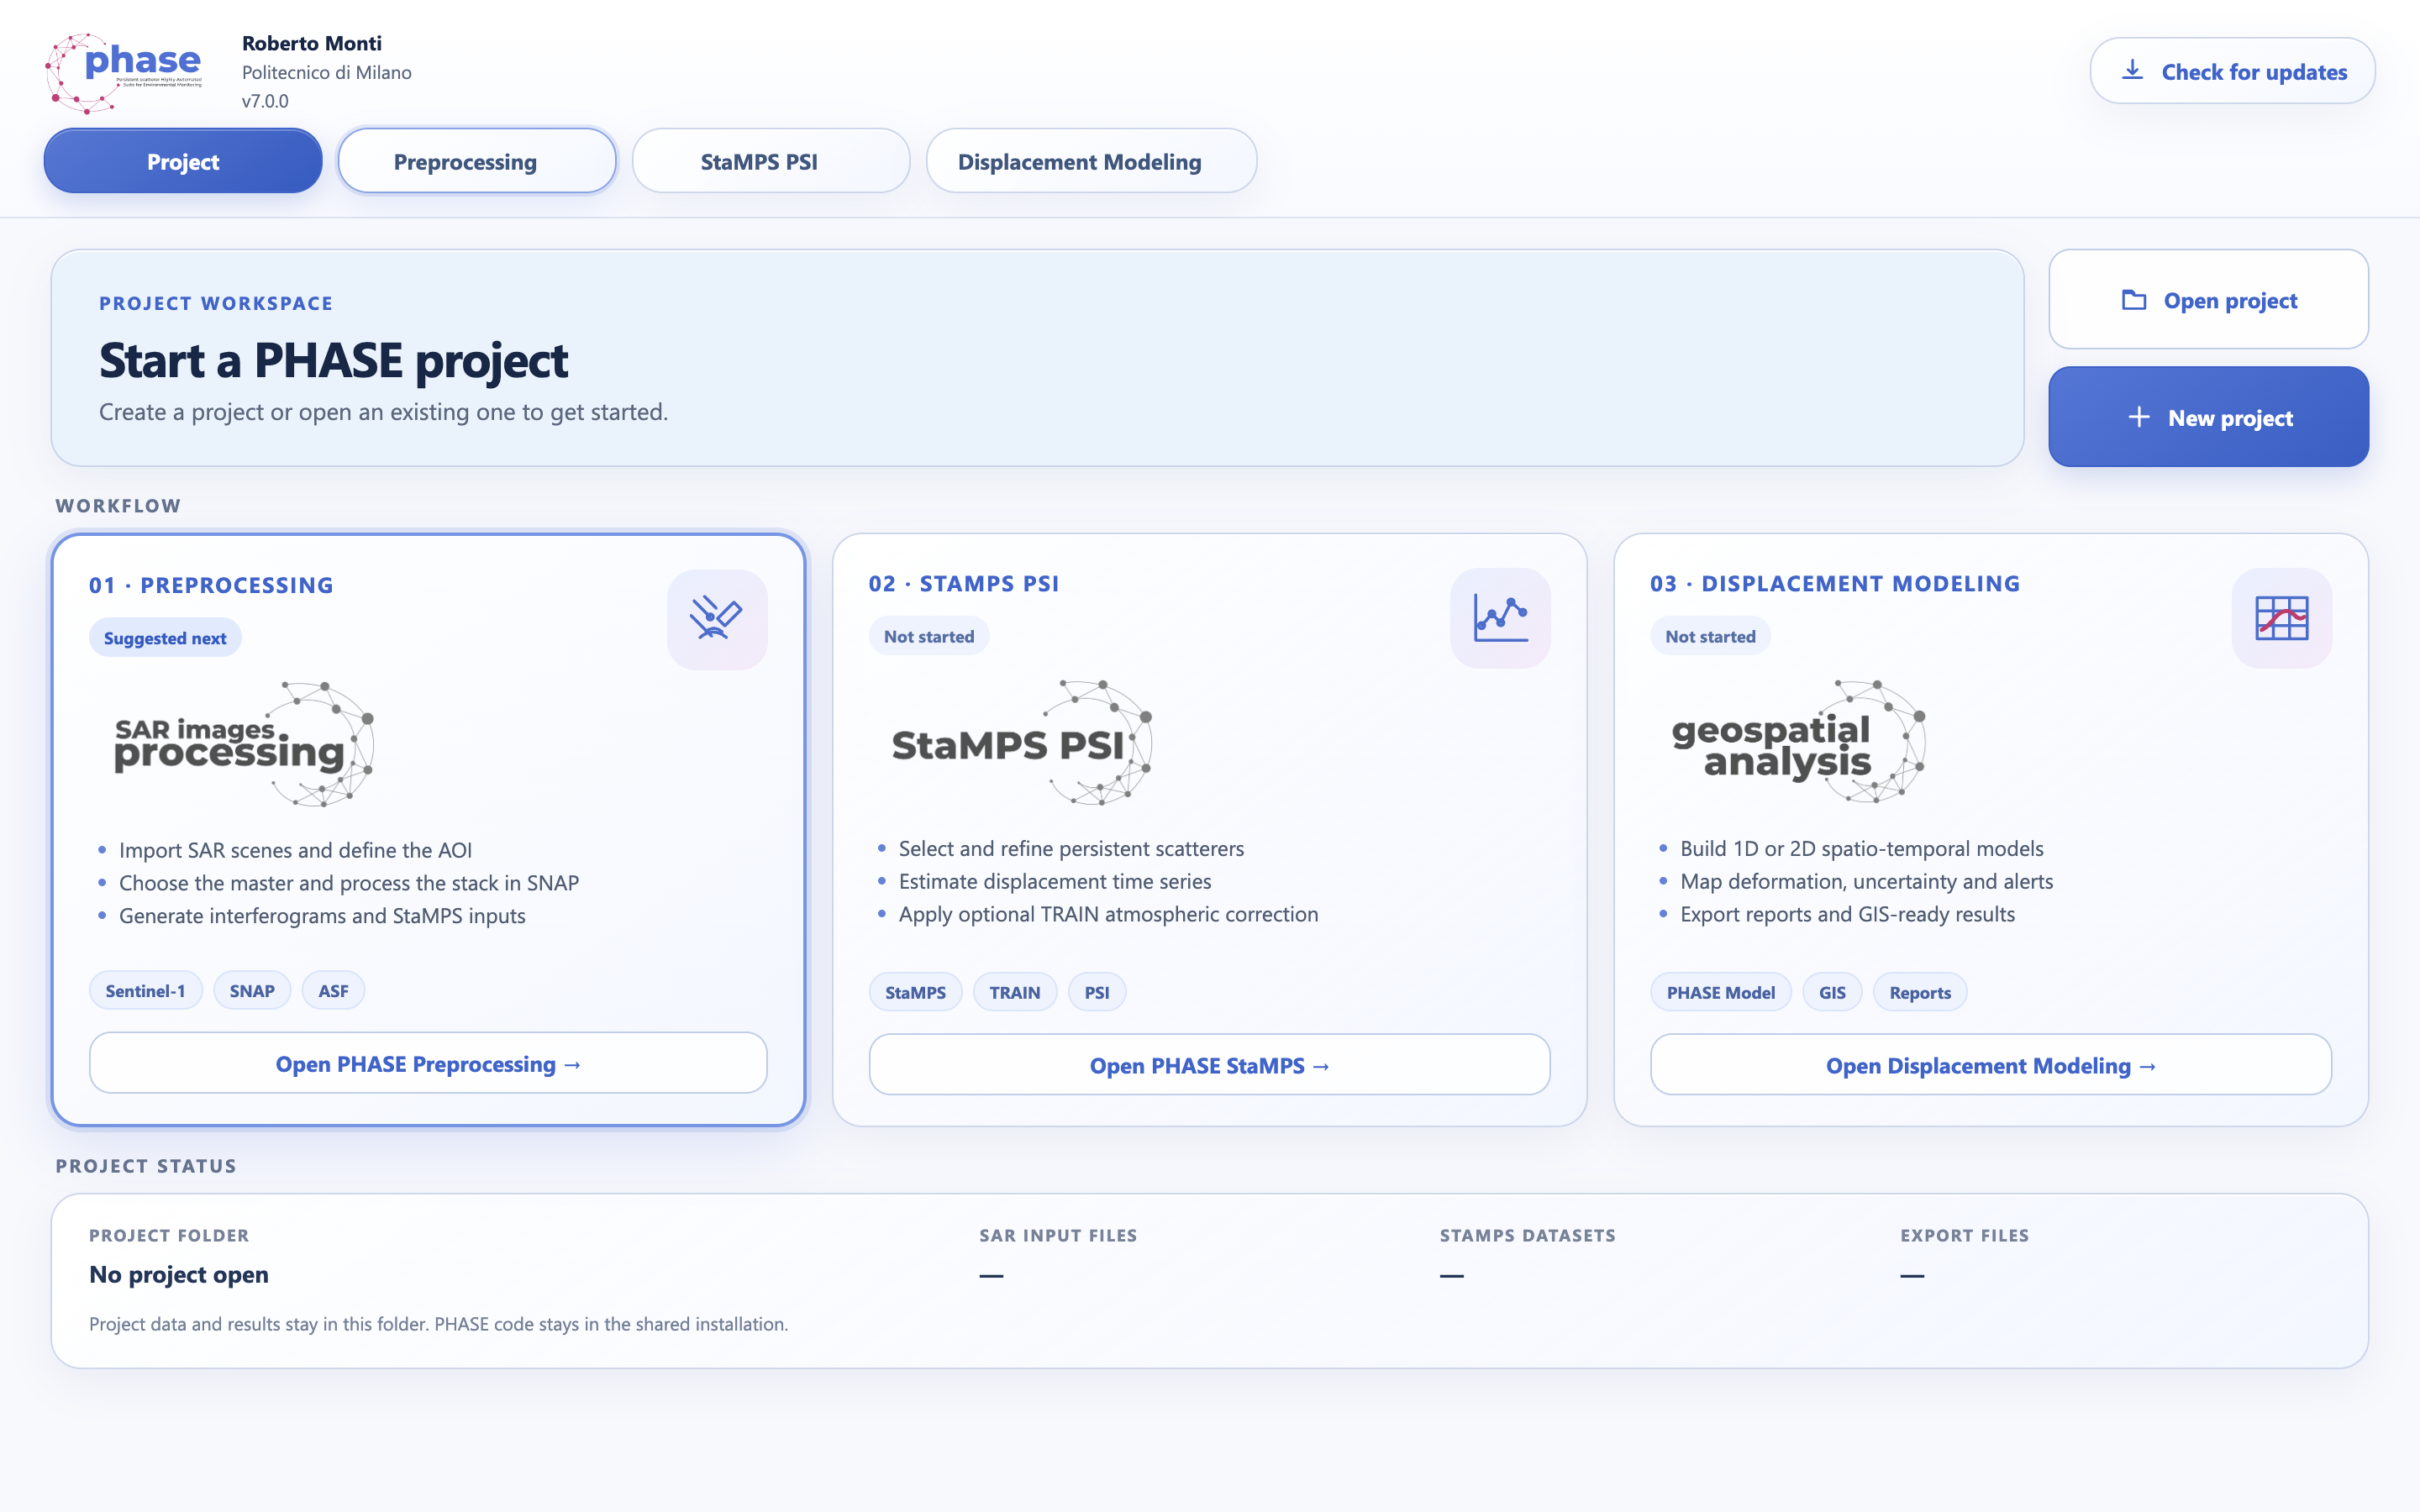
\includegraphics[width=\textwidth]{images/Screenshot 2026-10-11 alle 23.03.21.png}
    \caption{PHASE 7 hub before opening a project. The four navigation buttons, workflow cards, project actions and update control are part of one application.}
    \label{fig:phase7-hub}
\end{figure}

\noindent New projects use this top-level structure:
\begin{description}[leftmargin=3.3cm,style=nextline]
    \item[\texttt{01\_INPUT}] User-supplied SAR archives and AOI input files.
    \item[\texttt{02\_PROCESSING\_INTERNAL}] Intermediate SNAP and StaMPS work products. Do not modify while a run is in progress.
    \item[\texttt{03\_RESULTS}] Final PSI time series, modeling products, figures, GIS data and reports.
    \item[\texttt{04\_LOGS}] Execution logs and, if applicable, a legacy-import catalog.
\end{description}

Existing projects retain their original folder names because processing state may refer to those paths. In the hub, a green stage indicator means PHASE found outputs for that stage; it does not certify scientific quality. The highlighted stage is a suggested next action. Use \textbf{Check for updates} to download a compatible stable engine; close and relaunch PHASE to apply it. Projects and installed StaMPS/TRAIN runtimes are kept separate from the update. See the release notes for update availability and platform-specific instructions.

%\vspace{\baselineskip}
\subsection*{References and acknowledgments}
\noindent When utilizing PHASE Module 1 for your research, please ensure you refer to and cite the foundational works that make this pipeline possible:
\begin{itemize}
    \item \bibentry{monti2025phase}
    \item \bibentry{foumelis2018snap}
    \item \bibentry{hooper2008multi}
    \item (if TRAIN is used) \bibentry{bekaert2015statistical}
\end{itemize}

\vspace{\baselineskip}
\noindent The Authors express their gratitude to Jose Manuel Delgado Blasco and Dr. Michael Foumelis for the development of the snap2stamps tool and Prof. Andy Hooper for the development of StaMPS.

\part{Module 1}
\chapter{SAR images preprocessing}

\begin{figure}[H]
\centering
\includegraphics[width=0.8\columnwidth]{images/PHASE_mod1a.png}
\end{figure}

\section{Purpose and prerequisites}
The \textbf{Preprocessing} section prepares Sentinel-1 or COSMO-SkyMed scenes for StaMPS PSI. It handles image import or Sentinel-1 download, area-of-interest (AOI) definition, master selection, SNAP processing, interferogram formation, and StaMPS input export. It uses the shared PHASE installation; no project-local \texttt{.mlapp} or \texttt{snap2stamps} copy is required.

Install the PHASE release for your operating system and satisfy its checks for MATLAB, SNAP and the configured Python environment. Keep enough free storage for the SAR archives and substantially larger intermediate SNAP products. The first processing run may also need network access for orbit and elevation data. SNAP and external services are maintained independently of PHASE; if a download fails, inspect the \textbf{Run monitor} and the project logs before restarting.

\begin{quote}
\textcolor{orange}{\textbf{Scientific caution:}} The successful completion of a run means that the software finished, not that the interferograms are geodetically reliable. Inspect image overlap, orbit direction, burst coverage, coherence, phase quality, and the final AOI before proceeding to PSI.
\end{quote}

\section{Start a project}
Launch \textbf{PHASE}. Choose \textbf{New project} to create a workspace in any writable location, or \textbf{Open project} to resume one. The hub shows the project name, counts of input files, StaMPS datasets and exports, and the suggested next stage. Select \textbf{Preprocessing} from the hub navigation; the four section buttons remain available while working in a module. A green stage indicator is based on detected outputs and is not a data-quality assessment.

New projects separate input data, internal processing, final results and logs into four numbered top-level folders, as listed in the Introduction. PHASE creates the needed subdirectories. Do not rename or edit active processing directories, especially when resuming a stack. Older projects may retain their original layout.

\section{Images and AOI}
\subsection{Sentinel-1 download or import}
Use the module's \textbf{Download} section to search for and download Sentinel-1 scenes through the ASF service, or use \textbf{Import images} to add local archives. An ASF account and valid access may be required by the service. For a coherent stack, use compatible acquisition geometry, orbit direction, polarization, mode, and overlapping coverage. The map helps delimit the search and inspect the scene footprints; the later AOI controls what PHASE processes.

\begin{figure}[htbp]
\centering
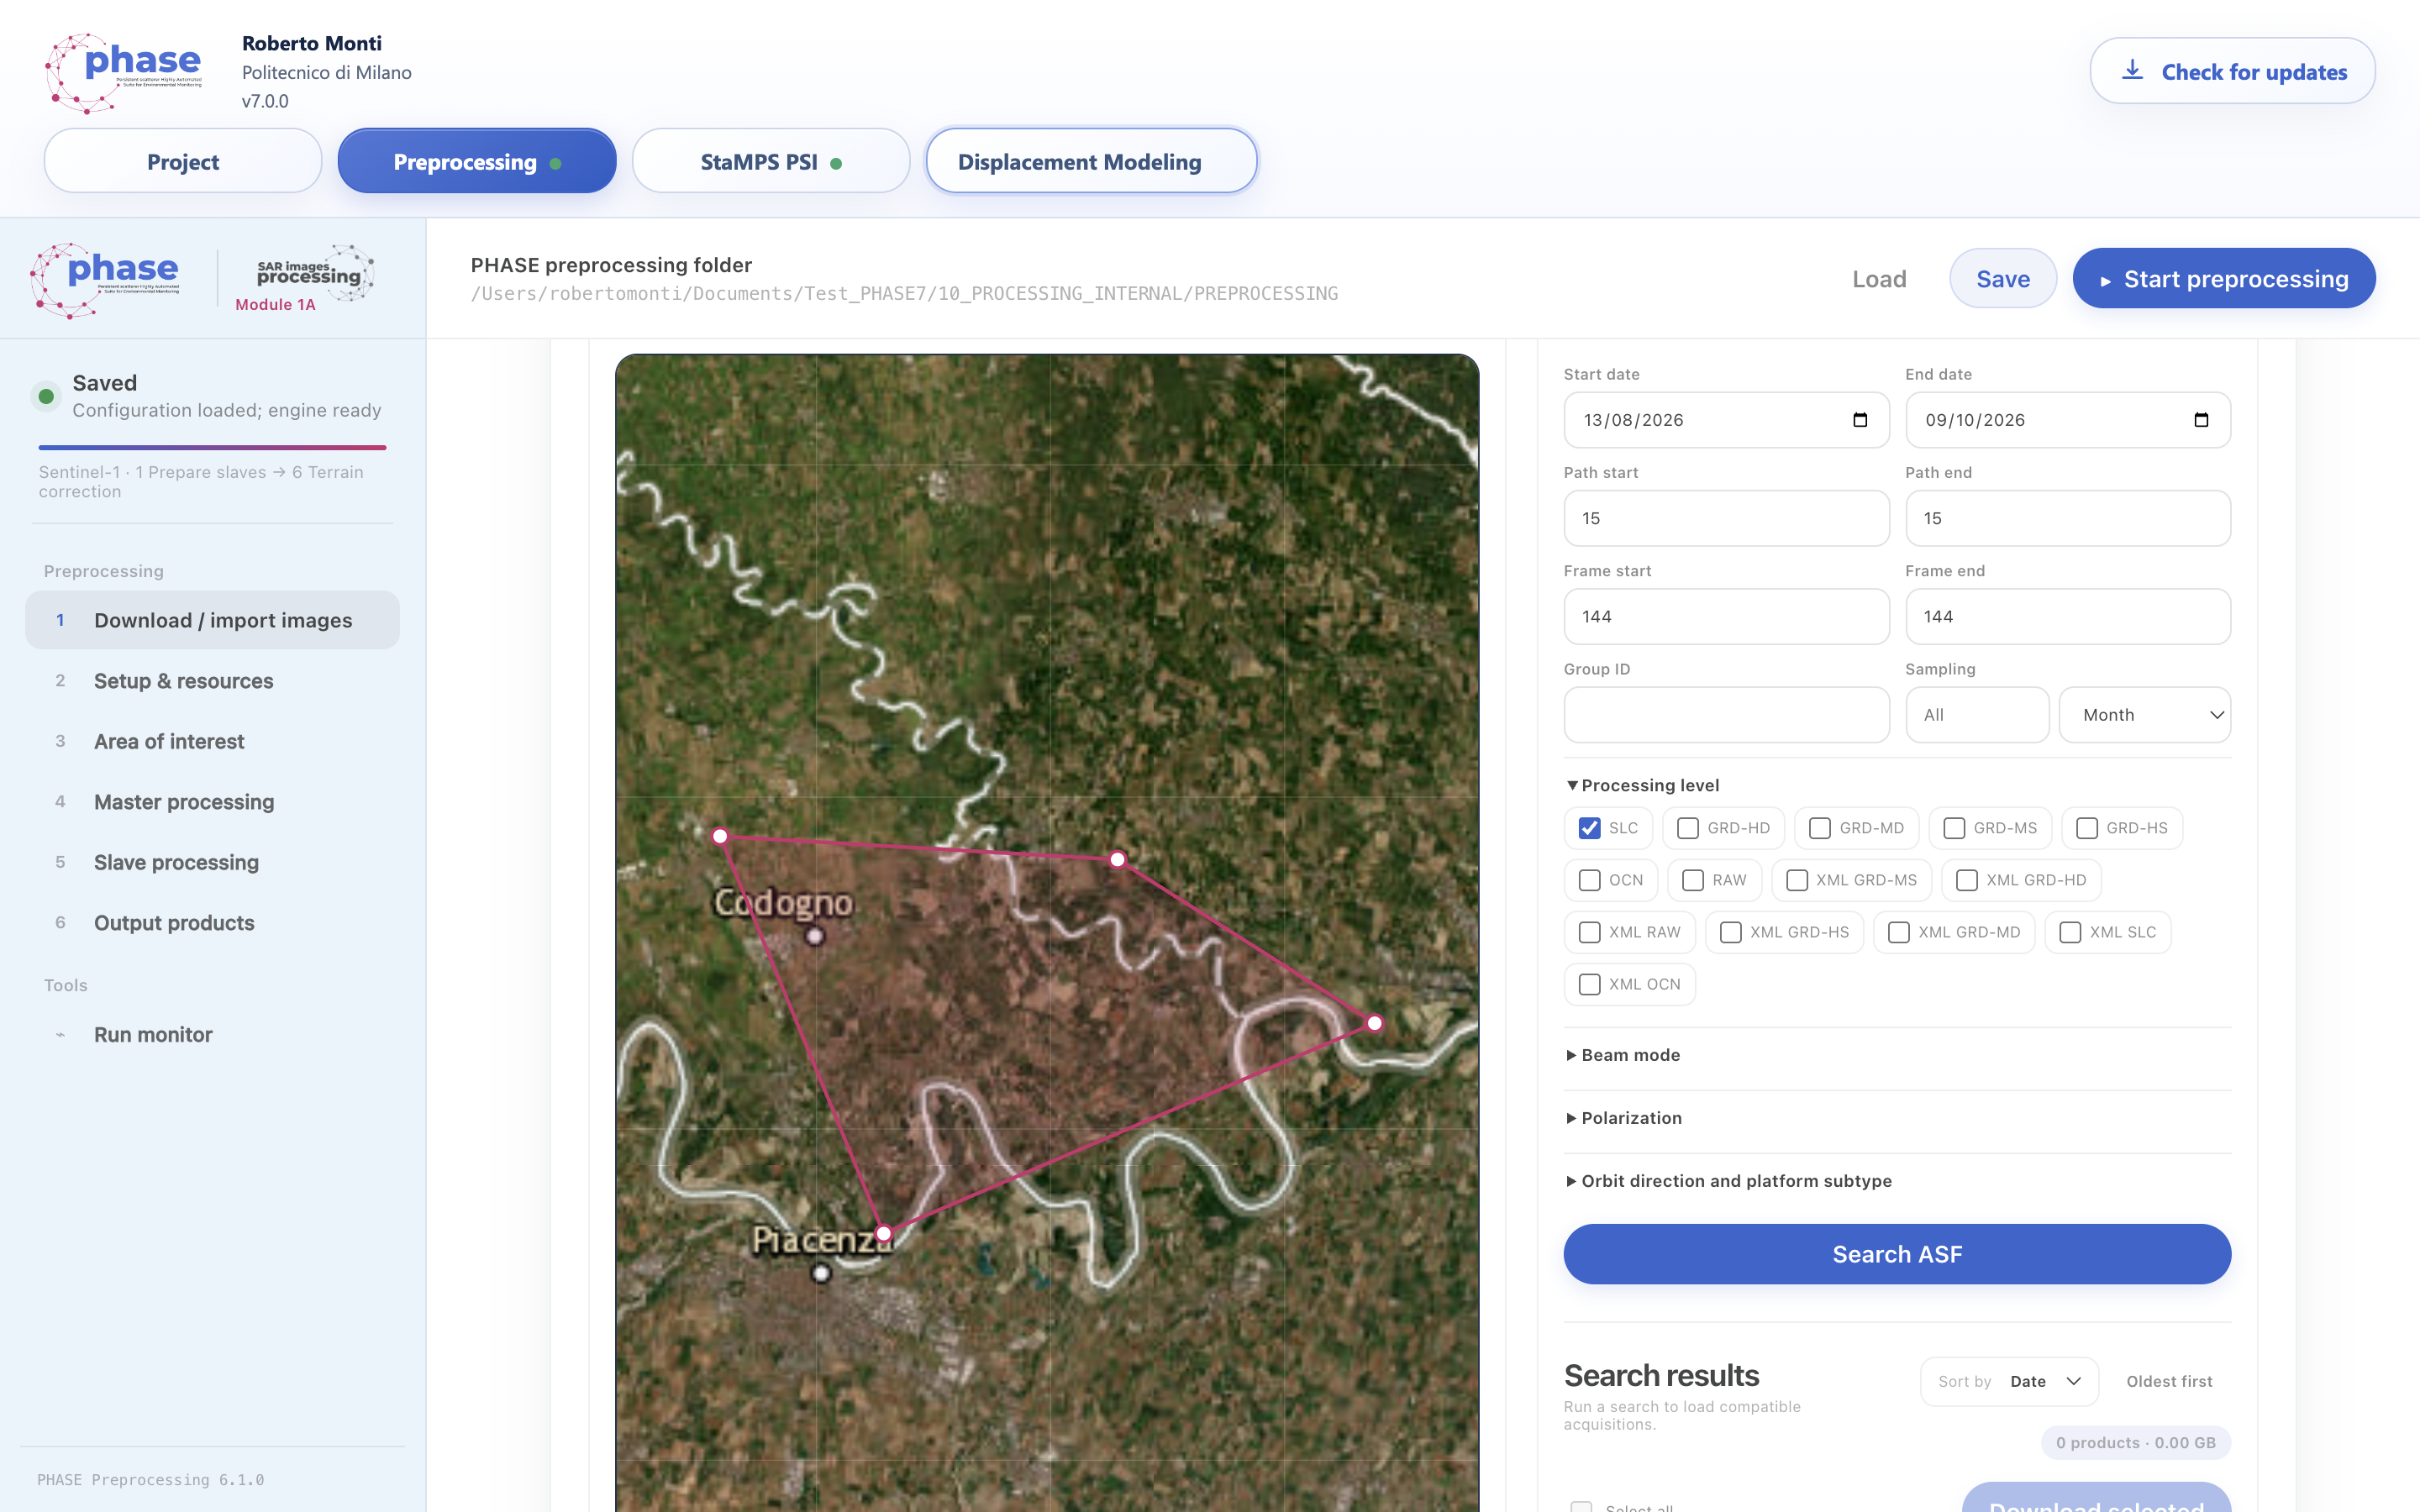
\includegraphics[width=\textwidth]{images/Screenshot 2026-10-11 alle 23.10.22.png}
\caption{Sentinel-1 search in the integrated Preprocessing section. The map and ASF filters are shown together; the displayed search parameters are examples, not recommended settings for every project.}
\label{fig:phase7-asf}
\end{figure}

For an existing Sentinel-1 stack, the \textbf{Update stack} workflow searches for and processes newly available compatible images while retaining existing products. Review its options and back up valuable results before a substantial reprocessing operation. Importing images from a different project is possible, but first confirm that they truly belong to the same geometry and acquisition series.

\subsection{COSMO-SkyMed scenes}
COSMO-SkyMed (CSK/CSG) scenes are obtained through the applicable data provider and imported locally. Check that the product type is supported by the selected preprocessing workflow and that the scenes share acquisition geometry and adequate AOI overlap. Access conditions, file formats, and mission-specific restrictions are controlled by the provider; consult its current documentation. PHASE does not convert an incompatible set of acquisitions into a valid interferometric stack.

\subsection{AOI selection}
Open the \textbf{Area of Interest} panel and draw the processing box on the map over the displayed footprint. Keep a margin around the target area so that registration and later quality checks have usable coverage. The selected geographic bounds are transferred to the processing parameters. A satellite basemap requires network access; if tiles are unavailable, verify the numerical bounds and footprint rather than assuming that a blank basemap means missing SAR coverage.

\begin{figure}[htbp]
\centering
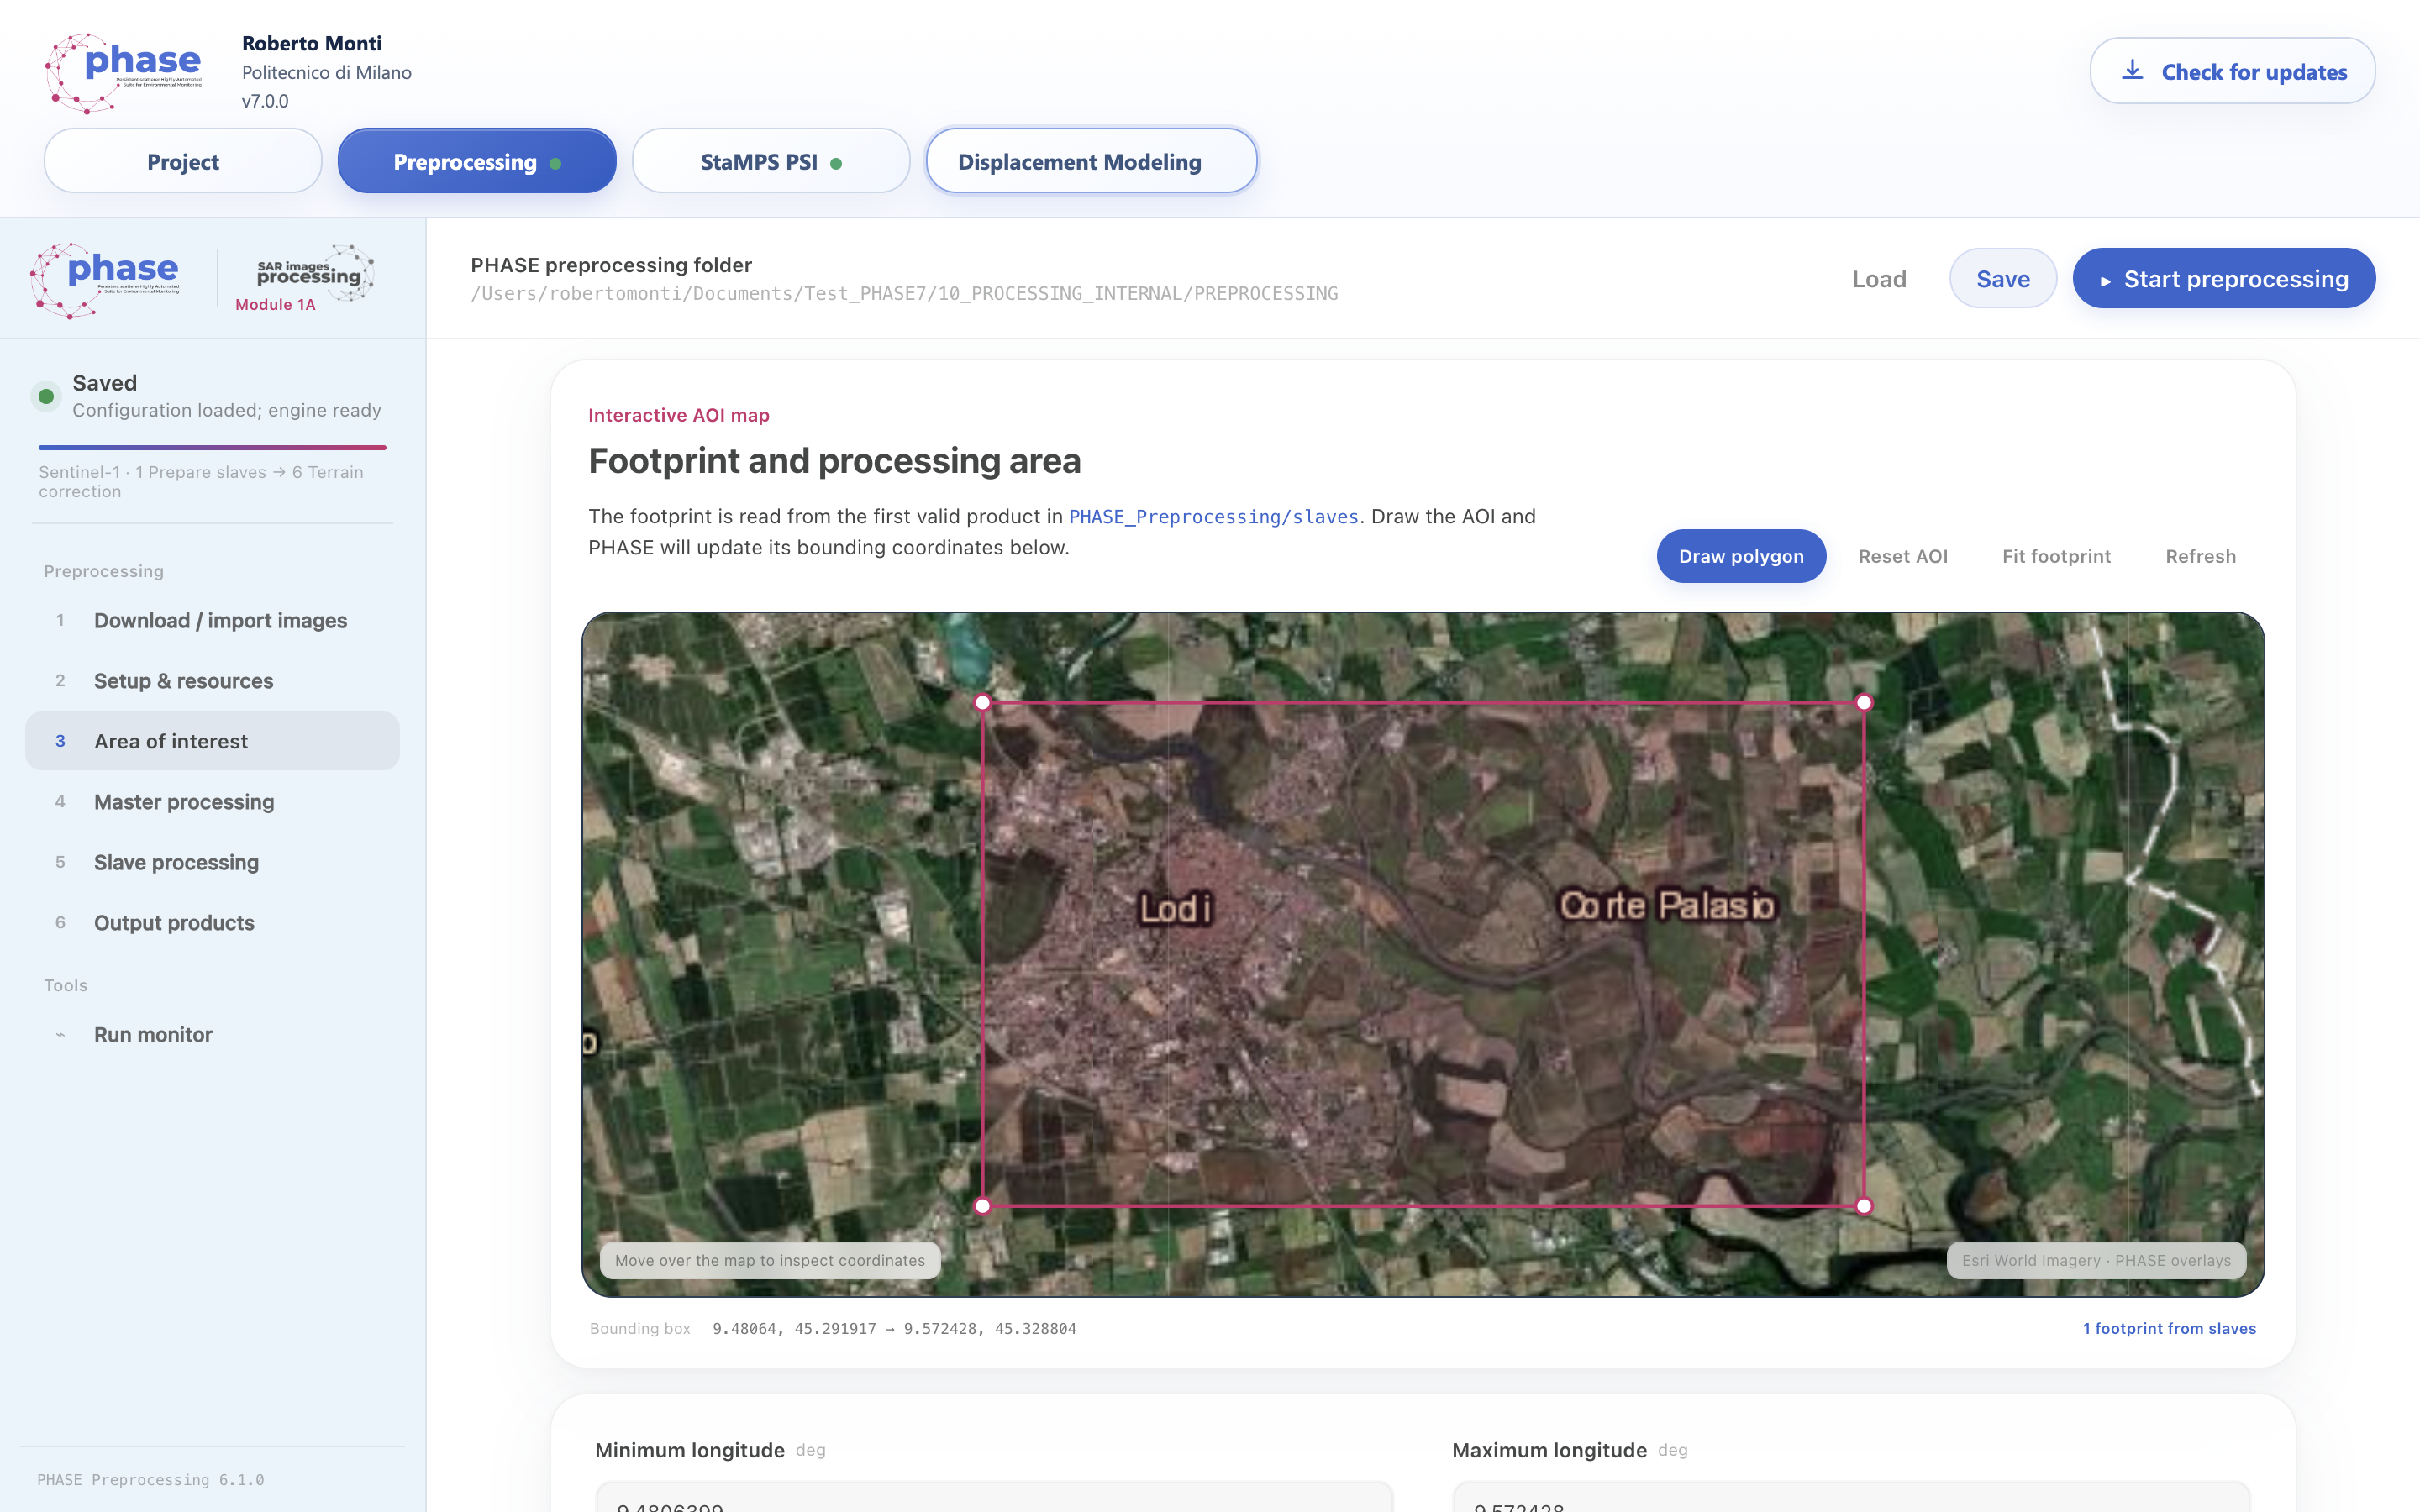
\includegraphics[width=\textwidth]{images/Screenshot 2026-10-11 alle 23.10.41.png}
\caption{Interactive processing AOI in PHASE 7. The pink polygon and numerical bounds illustrate the area selected for this example project.}
\label{fig:phase7-aoi}
\end{figure}

\section{Master selection and parameters}
PHASE can propose a master based on the available stack. Review its position in time and spatial overlap. For manual selection, use the date picker: it is constrained to acquisition dates found in the imported slaves and writes the date in the format required by the processing engine. Do not type an arbitrary date that is absent from the stack. For Sentinel-1, PHASE derives the needed swath/burst choices from scene metadata and AOI; verify them when the footprint is marginal or crosses burst boundaries.

In the \textbf{Master processing}, \textbf{Slaves processing}, \textbf{Coherence and LIA}, and \textbf{Computational resources} sections, review the active controls before launching a run. SNAP's \texttt{gpt} location, memory, concurrency, temporary storage and DEM choice affect performance and reproducibility. PHASE applies platform-aware limits where available, but an unusually large AOI or stack can still exceed system resources. Reduce AOI or concurrency if repeated runs exhaust memory. Use an external DEM only after checking its reference system, NoData value and full spatial coverage (see Appendix A).

\section{Run and interpret progress}
Save the configuration, then choose \textbf{Start preprocessing}. The \textbf{Run monitor} shows the current operation, elapsed time, a progress estimate, the slave being handled and a live log. Major operations include split/orbit handling, coregistration, interferogram and topographic-phase processing, StaMPS export, average intensity, and optional coherence/local-incidence-angle outputs. A percentage is an estimate of completed operations, not a time-to-finish prediction; an individual SNAP operation may take much longer than its neighbors.

If a run fails, preserve its error log and identify the exact scene and operation before retrying. When resuming from a slave step, PHASE can reuse existing master products; do not remove those products manually unless the run monitor explicitly instructs you to start from scratch. When preprocessing finishes, return to the hub or open \textbf{StaMPS PSI} through the persistent navigation. PHASE does not launch a separate StaMPS app. Check the expected StaMPS dataset and interferogram count before starting PSI.

\section{Processing outline}
For Sentinel-1, the principal SNAP operations include TOPSAR splitting and orbit application, back-geocoding and optional enhanced spectral diversity, interferogram formation, debursting, topographic-phase removal, StaMPS export, and terrain-corrected auxiliary layers. COSMO-SkyMed follows its own subset, stack, registration, interferogram and export path. The order and optional operations depend on the selected configuration; the run log is the authoritative record for a specific project.

\section{Troubleshooting}
\begin{description}[style=nextline]
\item[Missing basemap] Verify internet access and tile-service availability. Continue only after independently checking AOI coordinates and footprint.
\item[Orbit or DEM download failure] Check external-service connectivity and SNAP logs. If appropriate, provide a verified external DEM. Avoid treating an incomplete orbit/DEM step as a successful run.
\item[SNAP memory or process failure] Reduce simultaneous workers, AOI or stack size and confirm adequate free disk space. Keep the error log so that a reproducible failure can be distinguished from transient resource pressure.
\item[No suitable master or burst overlap] Recheck scene geometry, orbit direction, selected AOI and acquisition dates; do not force a non-overlapping master.
\end{description}

\chapter{StaMPS Persistent Scatterer Interferometry}

\begin{figure}[H]
\centering
\includegraphics[width=0.8\columnwidth]{images/PHASE_mod1b.png}
\end{figure}

\section{Open a prepared dataset}
After preprocessing, select \textbf{StaMPS PSI} in the same PHASE window. Choose the dataset from the selector at the top of the module; \textbf{Refresh} rescans the project's prepared datasets. The working directory is shown below it. The shared StaMPS and, when needed, TRAIN runtimes are installed with PHASE and remain outside the project folder. Do not move the applications or copy the runtime into individual projects.

Windows and macOS Apple Silicon have been exercised with end-to-end PSI runs. Linux is distributed with an experimental native build path, but a complete PSI run has not yet been independently validated there. Always review the current release notes and prerequisites before relying on a result.

\section{Configure the analysis}
The sidebar contains \textbf{Project}, \textbf{Global variables}, \textbf{Steps 1--8}, \textbf{Export}, \textbf{Run monitor} and \textbf{TS Points}. \textbf{Show all parameters} is enabled by default; hide advanced controls if you prefer a shorter view. Set the first and last StaMPS steps deliberately: the first full run normally includes data preparation and the steps needed for phase-noise estimation, PS selection, weeding, unwrapping, spatially correlated look-angle error estimation, and optional Step 8 filtering. A partial rerun depends on the preceding intermediate products.

\begin{figure}[htbp]
\centering
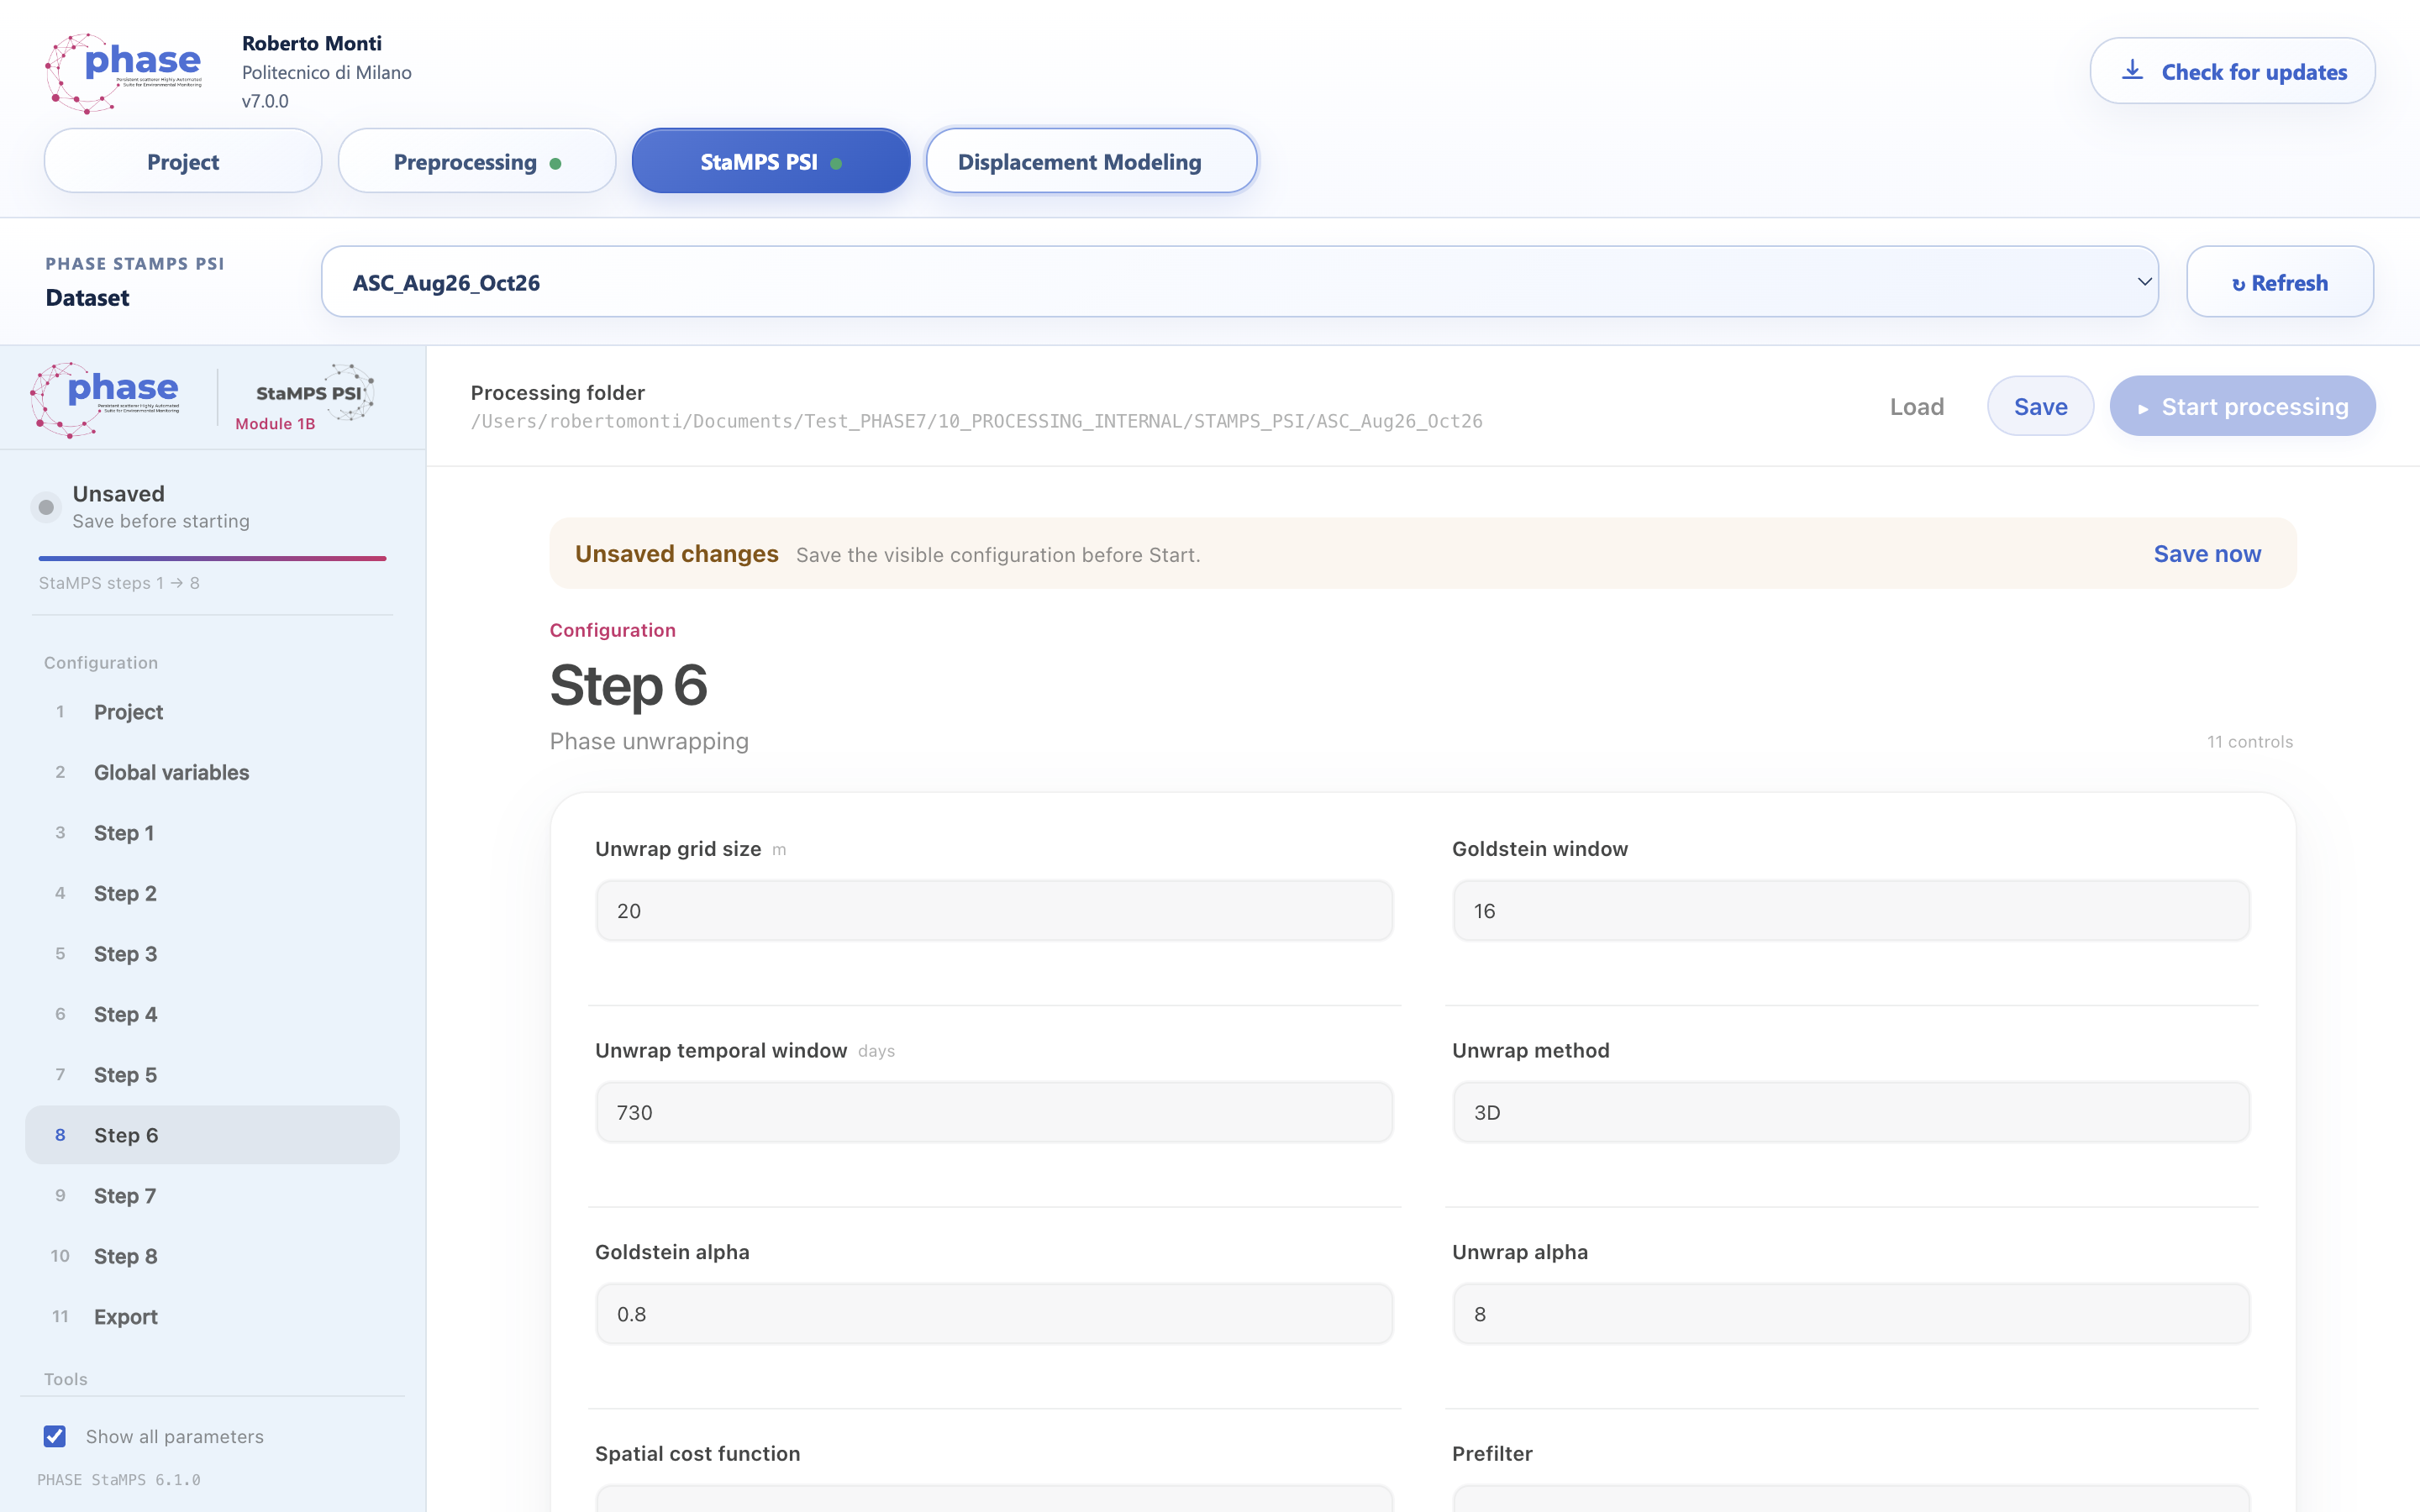
\includegraphics[width=\textwidth]{images/Screenshot 2026-10-11 alle 23.11.13.png}
\caption{StaMPS PSI within the unified hub. This example shows the Step 6 phase-unwrapping controls; the numerical values belong to the test project and should not be copied without analysis.}
\label{fig:phase7-stamps}
\end{figure}

PHASE detects key metadata where possible, including the master date and acquisition parameters. Inspect the automatically filled values against the source stack, especially after importing data from another processing system. The amplitude-dispersion threshold and phase-noise criteria control candidate density; relaxing them may increase the number of points while also adding noisy scatterers. Select a stable reference area or point appropriate for the study, because displacement is relative to a reference in space and time.

\subsection{Key StaMPS stages}
\begin{description}[style=nextline]
\item[Step 1 --- data preparation] Convert SNAP/StaMPS inputs and organize the interferogram stack.
\item[Steps 2--4 --- estimation and selection] Estimate phase noise, select PS candidates and remove inconsistent points.
\item[Steps 5--6 --- correction and unwrapping] Prepare corrected phase and unwrap it in space and time.
\item[Step 7 --- SCLA and ramp] Estimate spatially correlated look-angle/DEM error and, if configured, an orbital ramp.
\item[Step 8 --- spatially correlated noise] Optionally filter residual spatially correlated noise. Atmospheric delay can be a major component, but the Step 8 estimate is not guaranteed to be purely atmospheric and can absorb real spatially correlated deformation.
\end{description}

Consult the StaMPS manual for the scientific definition and interaction of individual parameters. PHASE presents them in a GUI but does not change their interpretation.

\section{Atmospheric correction and export choice}\label{ss:tropo}
PHASE offers an explicit \textbf{Standard} or \textbf{Corrected} displacement export. The choice controls both the automatic full CSV/XLSX series and the optional TS Points export. It is not inferred from whether the processing reached Step 8.

\begin{table}[htbp]
\centering
\caption{Displacement series exported through StaMPS \texttt{ps\_plot}.}
\begin{tabular}{@{}p{2.4cm}p{4.2cm}p{1.6cm}p{4.2cm}@{}}
\toprule
\textbf{Choice} & \textbf{Available source} & \textbf{Type} & \textbf{Additional subtraction at export} \\
\midrule
Standard & Step 7 or Step 8 & \texttt{v-do} & No additional \texttt{a} or \texttt{s} term \\
Corrected & TRAIN estimate available & \texttt{v-dao} & TRAIN tropospheric estimate, plus \texttt{d} and \texttt{o} \\
Corrected & No TRAIN; Step 8 completed & \texttt{v-dso} & Step 8 spatially correlated noise, plus \texttt{d} and \texttt{o} \\
\bottomrule
\end{tabular}
\end{table}

Here \texttt{d} denotes SCLA/DEM error and \texttt{o} an orbital ramp. Standard \texttt{v-do} means no \emph{additional} atmospheric subtraction in the export operation; it does not prove that no atmospheric effect was treated upstream. Corrected \texttt{v-dso} should be described as Step 8 spatial-noise-corrected, not as a pure atmospheric correction. If both TRAIN and Step 8 are configured, PHASE uses \texttt{v-dao} for the corrected export and does not silently combine the two estimates. If the requested TRAIN correction is unavailable, the corrected export fails rather than silently reverting to Standard.

TRAIN can be configured with a linear phase--topography model (\texttt{a\_linear}) or, when appropriate data are available, GACOS (\texttt{a\_gacos}). GACOS requires externally supplied atmospheric products and may pause the workflow while they are obtained; follow the paths and instructions displayed by the running application rather than an old, hard-coded folder example. Validate availability, date coverage and units before resuming. Correction can remove a geophysical component along with noise, so compare Standard and Corrected series when interpreting broad spatial signals.

\section{Run monitor and outputs}
Save the configuration and choose \textbf{Start processing}. The \textbf{Run monitor} displays the selected step range, correction and export summary, the current operation, a progress estimate, elapsed time and the processing log. Progress is based on StaMPS steps and patches; it is not proportional to elapsed time. Keep the run/error log for reproducibility, especially if native binaries or MATLAB stop unexpectedly.

PHASE automatically exports the complete point time series to CSV and XLSX. Displacements are in millimetres and velocity is in millimetres per year. The master epoch is the temporal zero; PHASE inserts a zero-valued master epoch only when it is absent from the StaMPS time axis. Export metadata record the chosen StaMPS value type in a \texttt{\_series.json} file. Inspect that metadata before comparing results produced with different correction modes. The exports are placed in the project's results area, while detailed processing files and logs remain separated.

The \textbf{TS Points} section and the \textbf{Explore TS Points} action in the Run monitor provide an \emph{optional} point-by-point inspection and selected-point export. They are not necessary to obtain the complete series. The picker is integrated into the StaMPS section and can be opened later from an already completed unwrapped PSI dataset. It uses the same export mode as the full series.

\begin{figure}[htbp]
\centering
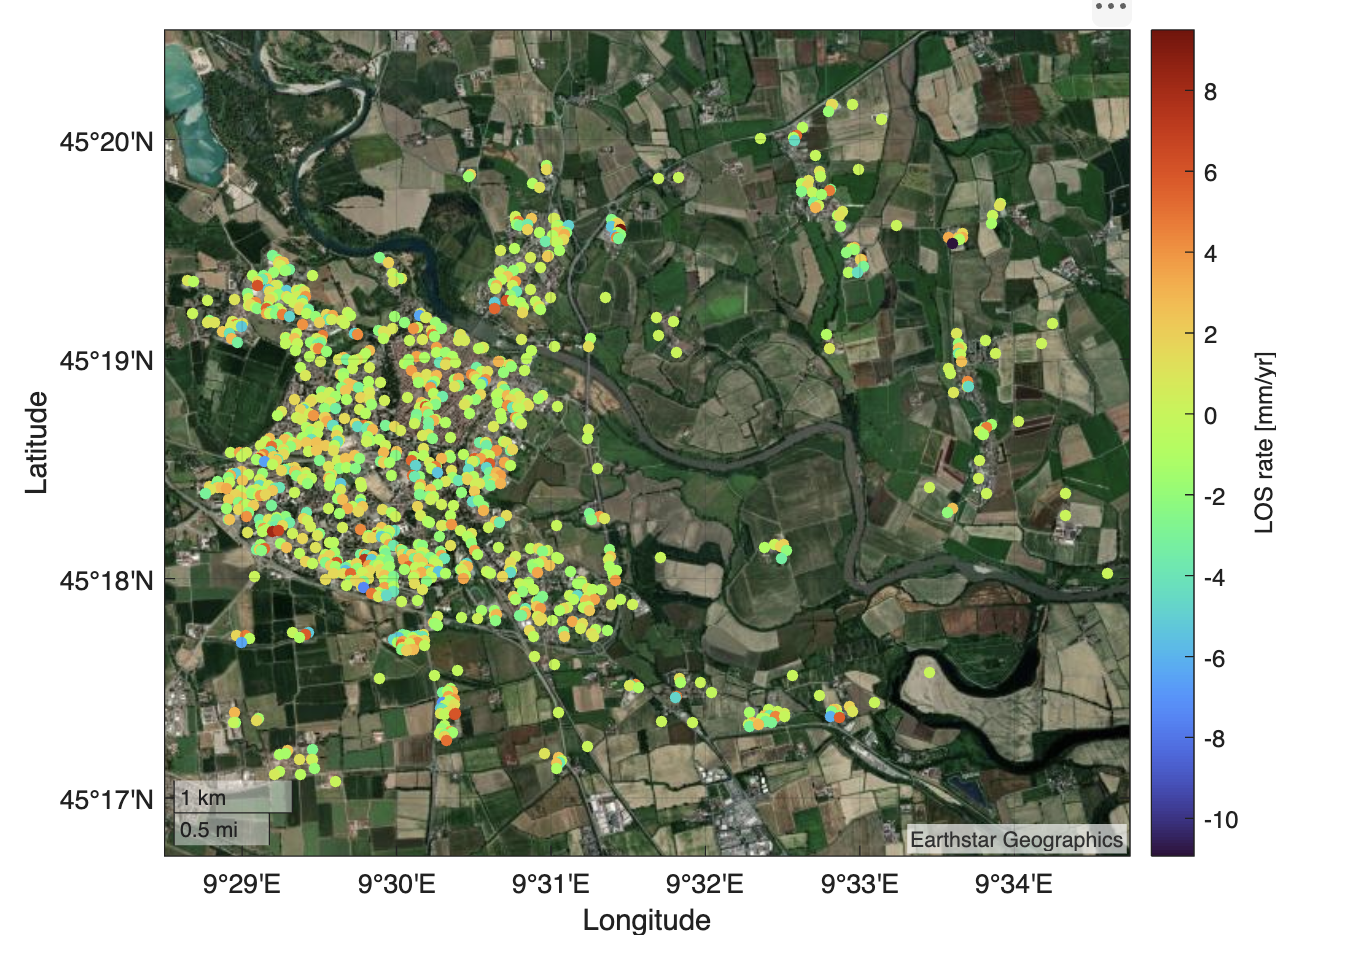
\includegraphics[width=0.9\textwidth]{images/PHASE_v7_PSI_output_example.png}
\caption{Example LOS velocity visualization from a PHASE 7 macOS PSI run. This operational test image does not independently validate the deformation estimates or establish the export correction mode.}
\end{figure}

\section{Quality checks and troubleshooting}
Before modeling, inspect the spatial distribution of PS points, temporal coverage, coherence/phase quality, the reference area and the sign and scale of LOS rates. Investigate large jumps, isolated outliers and differences between Standard and Corrected series; a visually plausible map alone is insufficient validation. Compare with independent measurements where available.

\begin{description}[style=nextline]
\item[No prepared dataset] Return to Preprocessing and check that StaMPS inputs were exported successfully; then use \textbf{Refresh}.
\item[Step 1 native-tool or Python error] Save the complete run log and verify that the installed PHASE runtime and prerequisites are accessible. Avoid modifying the shared runtime or project data without identifying the failing command.
\item[Correction unavailable] Confirm the selected TRAIN/GACOS inputs or complete Step 8 if using its correction. Do not interpret a Standard fallback as a corrected series.
\item[Unexpected point count] Revisit amplitude-dispersion and PS-selection settings, but avoid increasing density without checking noise and unwrapping quality.
\end{description}


\part{Module 2}
\chapter{Spatio-temporal modeling of PSI displacements}

\begin{figure}[H]
\begin{center}
		
\includegraphics[width=0.8\columnwidth]{images/PHASE_mod2.png}
\end{center}
\end{figure}

\section{Preliminary steps}

The \textbf{Displacement Modeling} section of the PHASE hub performs interpolation and modeling of PS time series generated by StaMPS PSI. It can also use externally generated PSI data when the input tables follow the expected format. Open it through the persistent hub navigation; do not copy a standalone \texttt{.mlapp} into a project.

The application requires MATLAB and the Python environment configured by the PHASE installation. Report generation uses Python packages such as \texttt{openpyxl} and \texttt{pillow}; use the installer's checks and the run log to diagnose missing packages.

\begin{quote}
    \textcolor{cyan}{\textbf{SUGGESTION:}} \textcolor{gray}{If Python integration fails, compare the Python interpreter shown by MATLAB's \texttt{pyenv} with the interpreter configured by the PHASE installer. Installing a package into a different Python environment will not fix the active runtime.}
\end{quote}

\noindent Some geospatial modeling operations can be highly computationally expensive. If the execution takes too long or exceeds your system's memory, you should try reducing the spatial resolution of the requested output grid.

\begin{quote}
    \textcolor{orange}{\textbf{WARNING:}} \textcolor{gray}{Please remember that all provided InSAR displacements are measured strictly along the satellite Line-of-Sight (LOS), which is a 1D vector.  The software models this specific 1D deformation and does not inherently decompose it into true vertical or horizontal 3D vectors.}
\end{quote}

This module of PHASE requires the following MATLAB packages to be installed:
\begin{itemize}
    \item Curve Fitting Toolbox.
    \item Image Processing Toolbox.
    \item Mapping Toolbox.
    \item Optimization Toolbox.
    \item Parallel Computing Toolbox.
    \item Signal Processing Toolbox.
    \item Statistics and Machine Learning Toolbox.
\end{itemize}

\section{Required folder structure}

PHASE code remains in the shared installation. Select or create a project in the hub, open \textbf{Displacement Modeling}, and point the module at the desired PSI output within \texttt{03\_RESULTS} (or at a compatible external dataset). Modeling output belongs to the project results area. Existing projects may use their original folder names.

\section{Description of the MATLAB application}
This stage takes scattered PS time series generated by StaMPS PSI (or external PSI processors) and converts them into temporal or spatio-temporal models and reports. The scientific options below remain relevant to the version 7 module; control placement may differ slightly from older PHASE releases.

\subsection{Input files}
Select the PSI output spreadsheet (\texttt{.xlsx} or \texttt{.csv}) and confirm the Python interpreter if prompted. For PHASE-generated series, check the adjacent \texttt{\_series.json} metadata so that you know whether the input is Standard \texttt{v-do}, TRAIN-corrected \texttt{v-dao}, or Step 8-corrected \texttt{v-dso}; these are scientifically different inputs.

Additionally, the date of the first observation in the time series must be specified. There is also a checkbox to automatically remove all the previous output folders prior to the software execution.


\subsection{Area of interest}
The second step involves defining the AOI, which delineates the spatial boundaries for computing and modeling displacements. This AOI can be specified on the map or by a shapefile. A shapefile must include a readable \texttt{.prj} defining WGS84 geographic coordinates or a WGS84-based projected CRS; coordinates are never guessed from their numeric range. PHASE projects the AOI, PS and optional query points into one common UTM CRS. If the AOI crosses two adjacent UTM zones, it chooses the zone covering the larger part of the AOI. Very wide, polar, equator-crossing and antimeridian-crossing AOIs require a different projection and are rejected explicitly rather than processed with inconsistent coordinates. Points outside the AOI are filtered to focus processing only on relevant PS.


\subsection{Processing options}

Depending on your analytical needs, the application allows you to choose between two alternative main processing modes, both of which conclude with automatic report generation:

\begin{description}[style=nextline]
    \item[Alternative 1: Temporal-only modeling (PS-by-PS)]
    This mode focuses strictly on the time domain without performing any spatial interpolation between points. The software automatically cleans and mathematically decomposes each individual PS time series. This includes: outlier removal, low-degree polynomial trend estimation, Fourier-based periodicity analysis, spline-based modeling of residual local components, and stochastic collocation on the residuals.

    \item[Alternative 2: Spatio-temporal modeling (interpolation)]
    This mode performs a joint spatio-temporal modeling, taking the scattered points data and interpolating them into continuous displacement fields. You can choose between two mathematical approaches (Deterministic splines or Stochastic Least Squares Collocation) across two spatial domains:
    \begin{itemize}
        \item \textbf{1D domain:} used when monitoring linear structures defined by a centerline (e.g., roads, railways, narrow arch dams).
        \item \textbf{2D domain:} used when monitoring wide, areal targets (e.g., cities, landslides, earth-filled dams).
    \end{itemize}

    \item[Final step: Automatic reporting]
    Regardless of which modeling path you choose, the module finalizes the process by generating a comprehensive Excel report (via Python integration) and reproducible, publication-ready maps. It also automatically applies thresholding to highlight specific areas exhibiting anomalous displacement behavior.
\end{description}

The overall flow of these processing options is schematized in the figure below.

\begin{figure}[H]
    \centering
    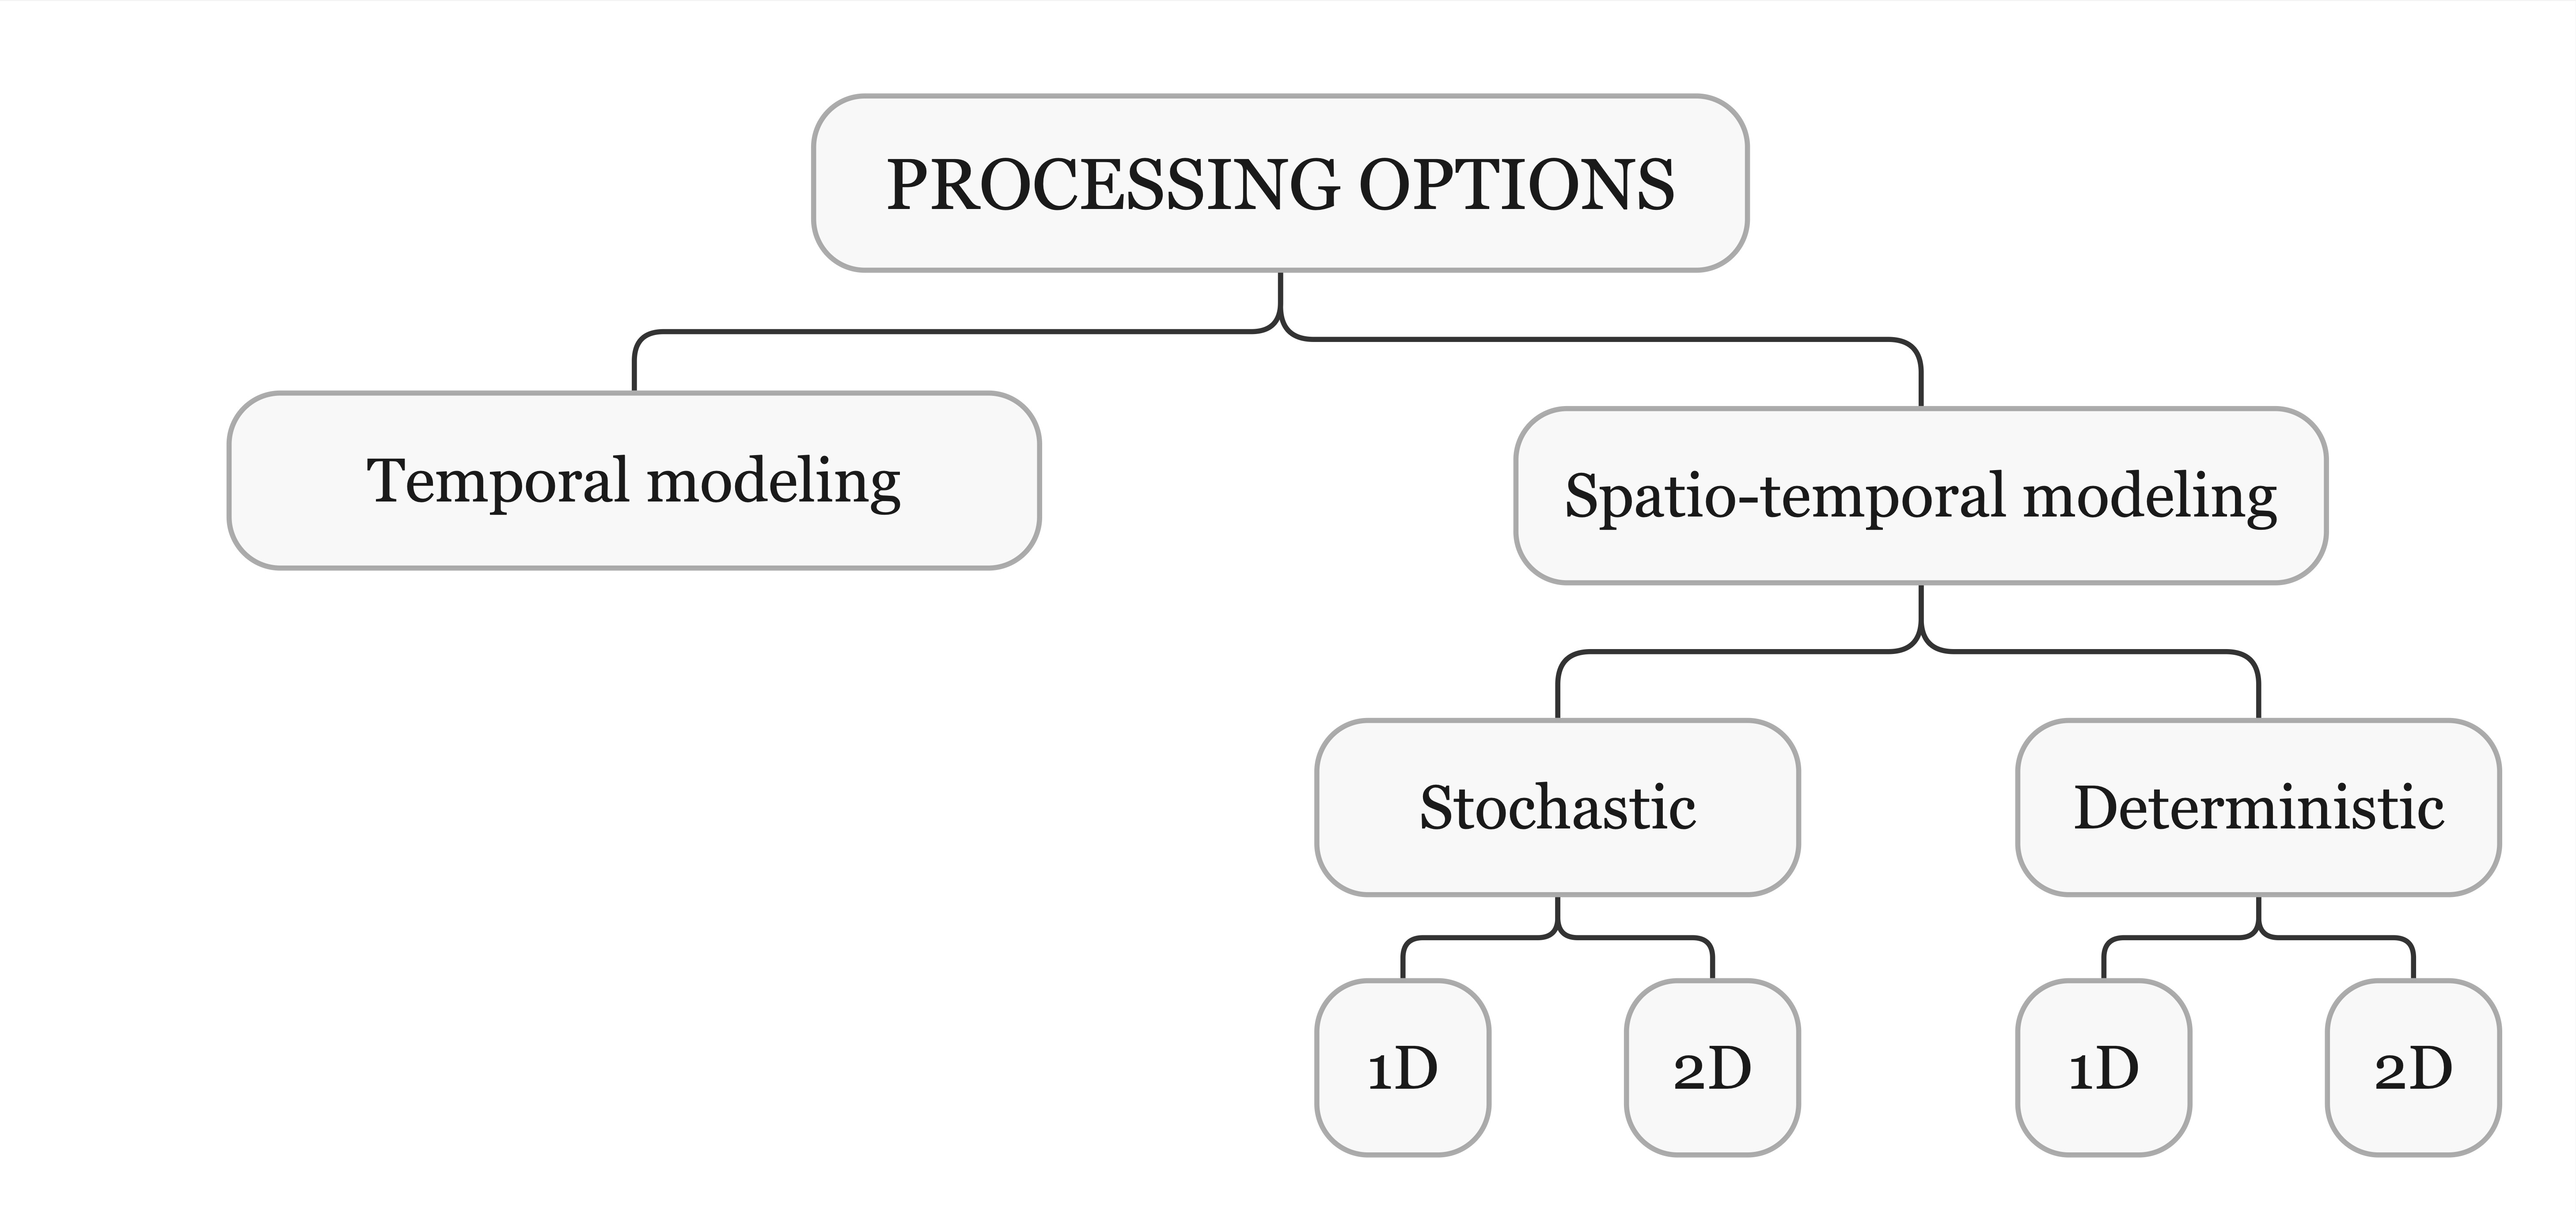
\includegraphics[width=0.9\textwidth]{images/Processing_options.jpg}
    \caption{Schematic representation of the processing options available in PHASE.}
\end{figure}

Consequently, the GUI has 4 available processing types:
\begin{itemize}
    \item \textbf{Temporal}: interpolation of all time series independently.
    \item \textbf{Temporal\&NNI}: interpolation of all time series independently and nearest neighbor spatial interpolation for visualization.
    \item \textbf{Spatio-temporalDET}: spatial interpolation with deterministic methodology.
    \item \textbf{Spatio-temporalSTC}: spatial interpolation with a joint deterministic and stochastic methodology.
\end{itemize}

\begin{figure}[htbp]
    \centering
    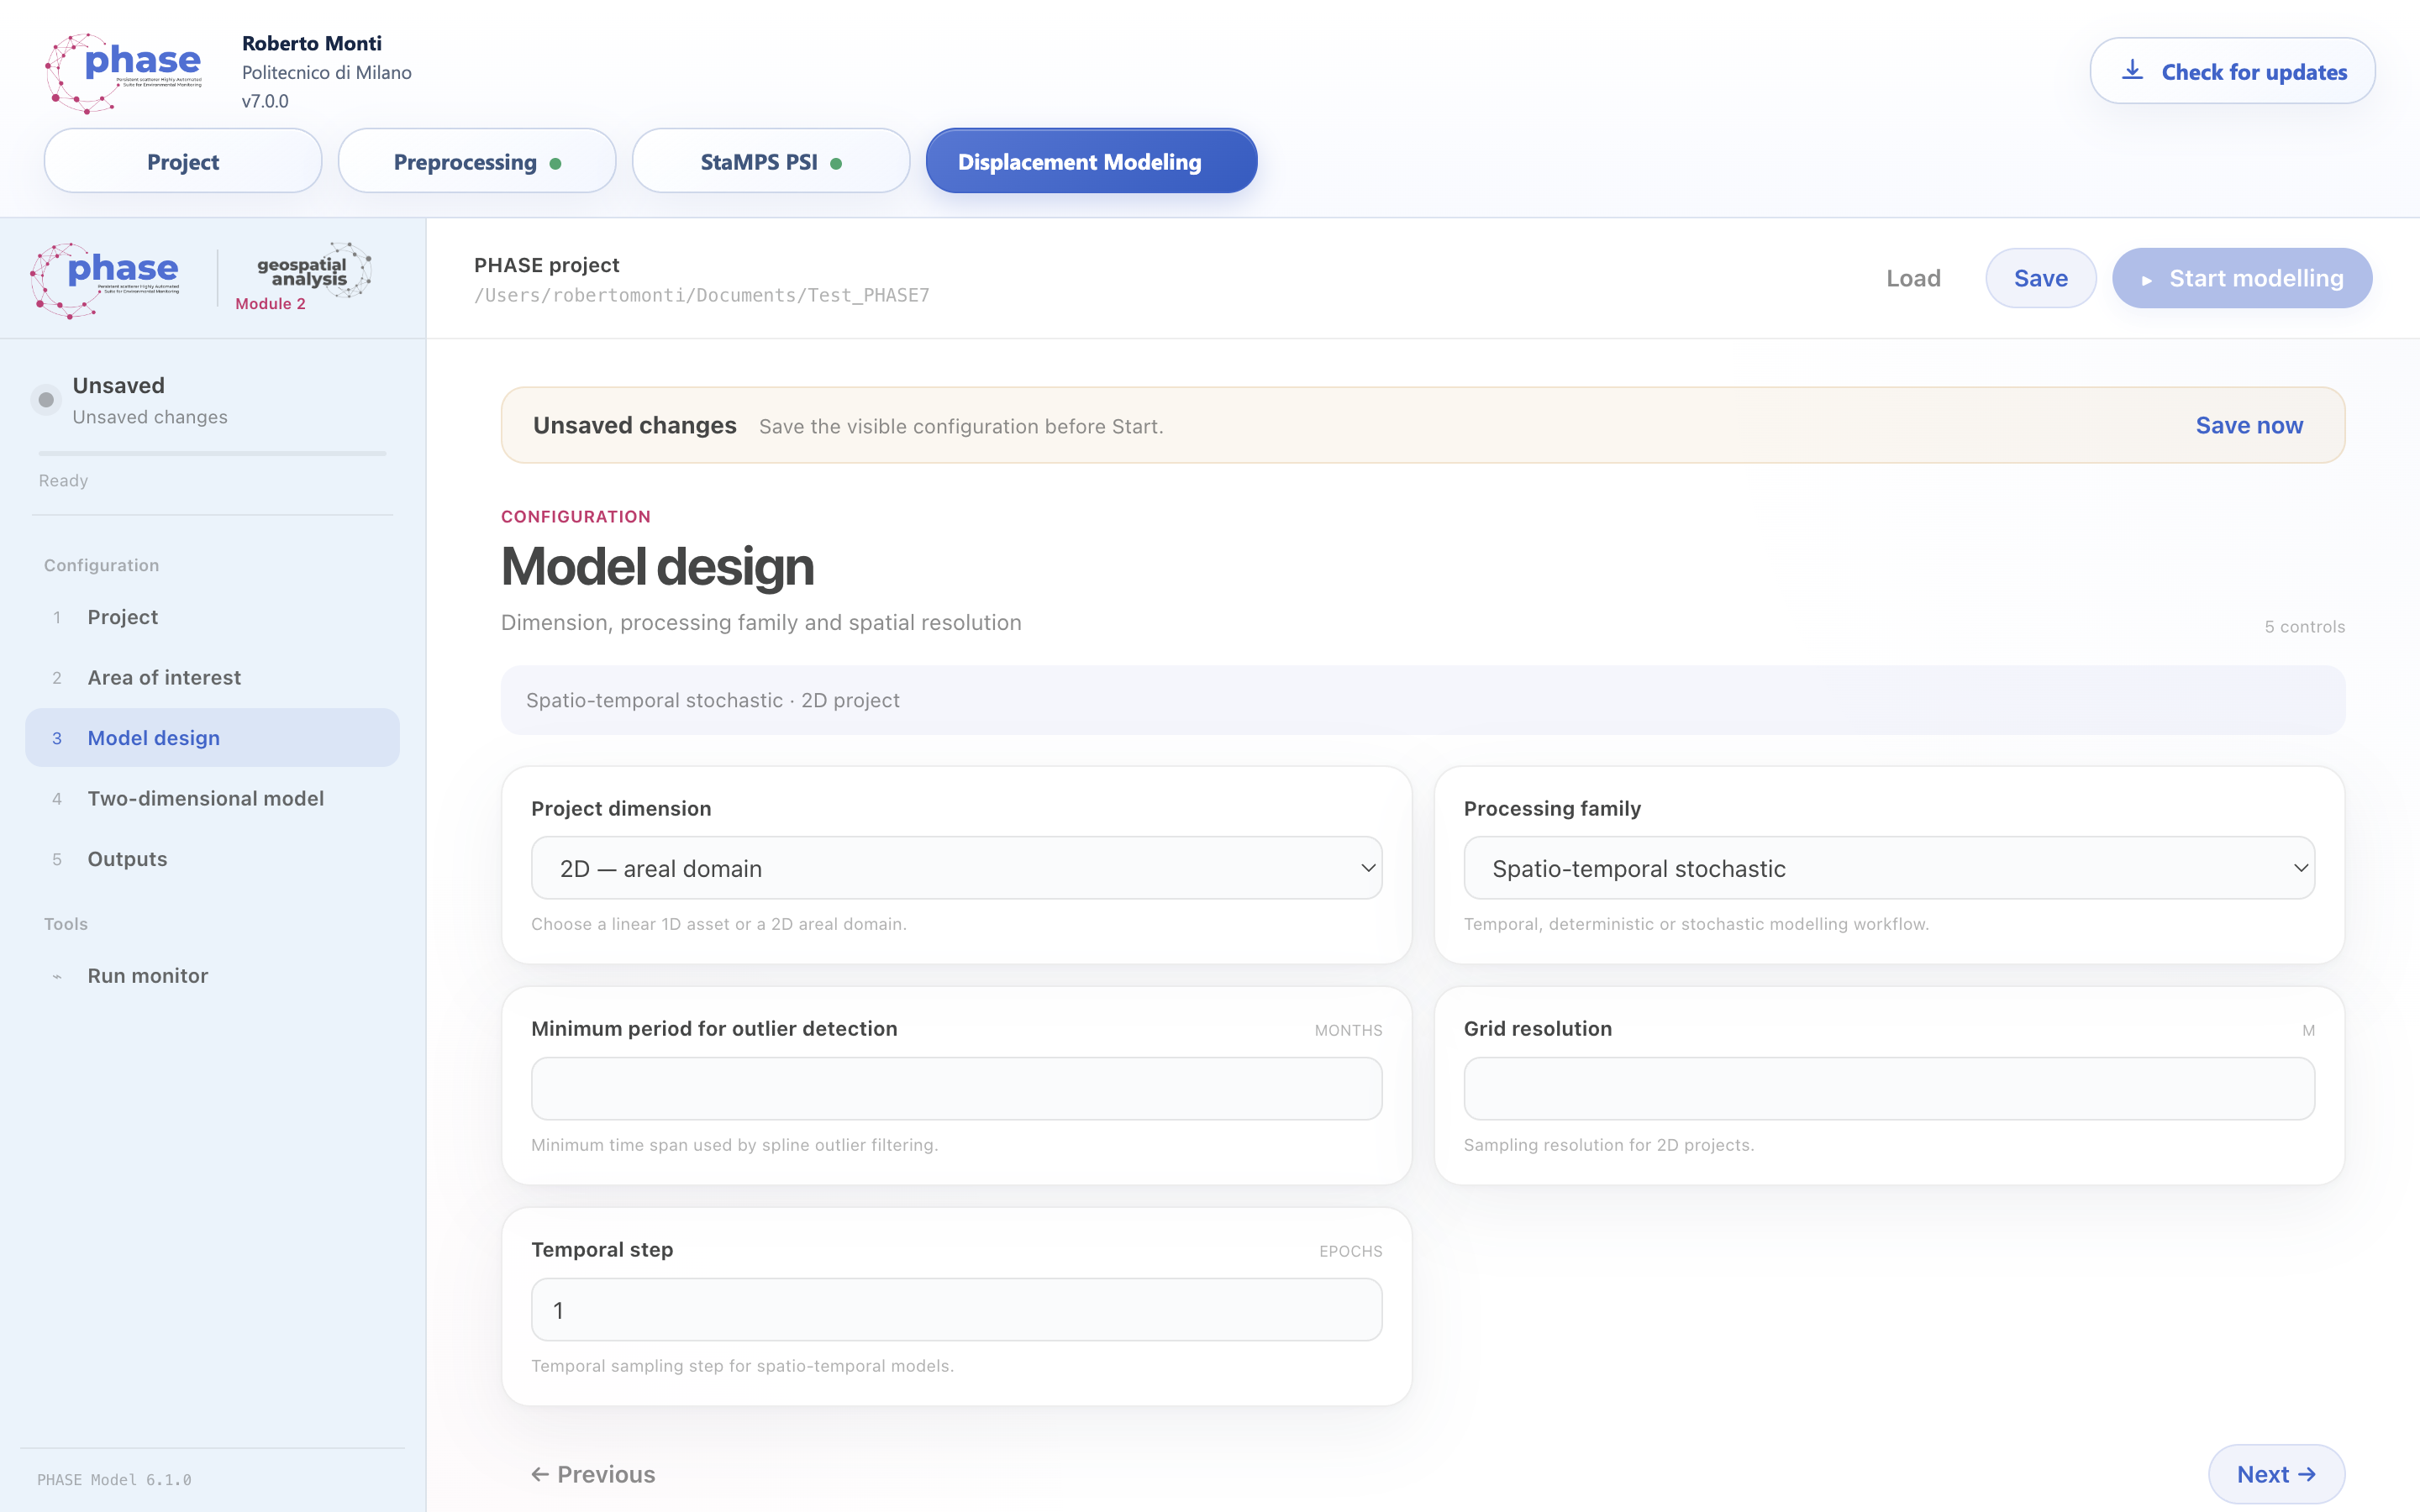
\includegraphics[width=\textwidth]{images/Screenshot 2026-10-11 alle 23.11.56.png}
    \caption{Model design in the PHASE 7 Displacement Modeling section. The example selects a two-dimensional spatio-temporal stochastic model; blank and unsaved controls in the screenshot are not a configuration to run as-is.}
    \label{fig:phase7-model-design}
\end{figure}

The following subsections explain how to configure each tab in the GUI.


\subsection{Temporal modeling}\label{ss:temp}
When the user selects the temporal-only mode, Module 2 performs a fully automated decomposition of every individual PS time series. The objective is to separate the physical deformation signal from background noise by modeling each scatterer independently, without influence from neighboring points.

\subsubsection{The configuration panel}
The temporal workflow is driven by a dedicated GUI section that centralizes the user-configurable parameters.

Through this interface, users can define the core parameters that govern the underlying mathematical estimators without needing advanced statistical expertise. Key selectable options include:
\begin{itemize}
    \item \textbf{A priori noise variance model:} choose between a coherence-based model, a constant manual value, or automatic estimation from the Fourier spectrum.
    \item \textbf{Spline knot number:} allow the software to automatically estimate the number of knots via statistical methods (variance threshold, MDL, F-test, $\chi^2$ test), or define them manually.
    \item \textbf{Regularization strength:} set the smoothing parameter $\lambda$ for the spline fit (automatic or user-defined).
    \item \textbf{Collocation strategy:} choose between filtering (estimation strictly at observation points) or prediction (interpolation).
    \item \textbf{Centerline/grid resolution:} define the resolution of the regular spatial domain for the estimation (\textit{available only if NNI is selected}).
\end{itemize}


\subsubsection{The processing workflow}
Once initiated, the software processes each PS through five sequential core stages, plus one optional spatial visualization stage.

\begin{figure}[H]
    \centering
    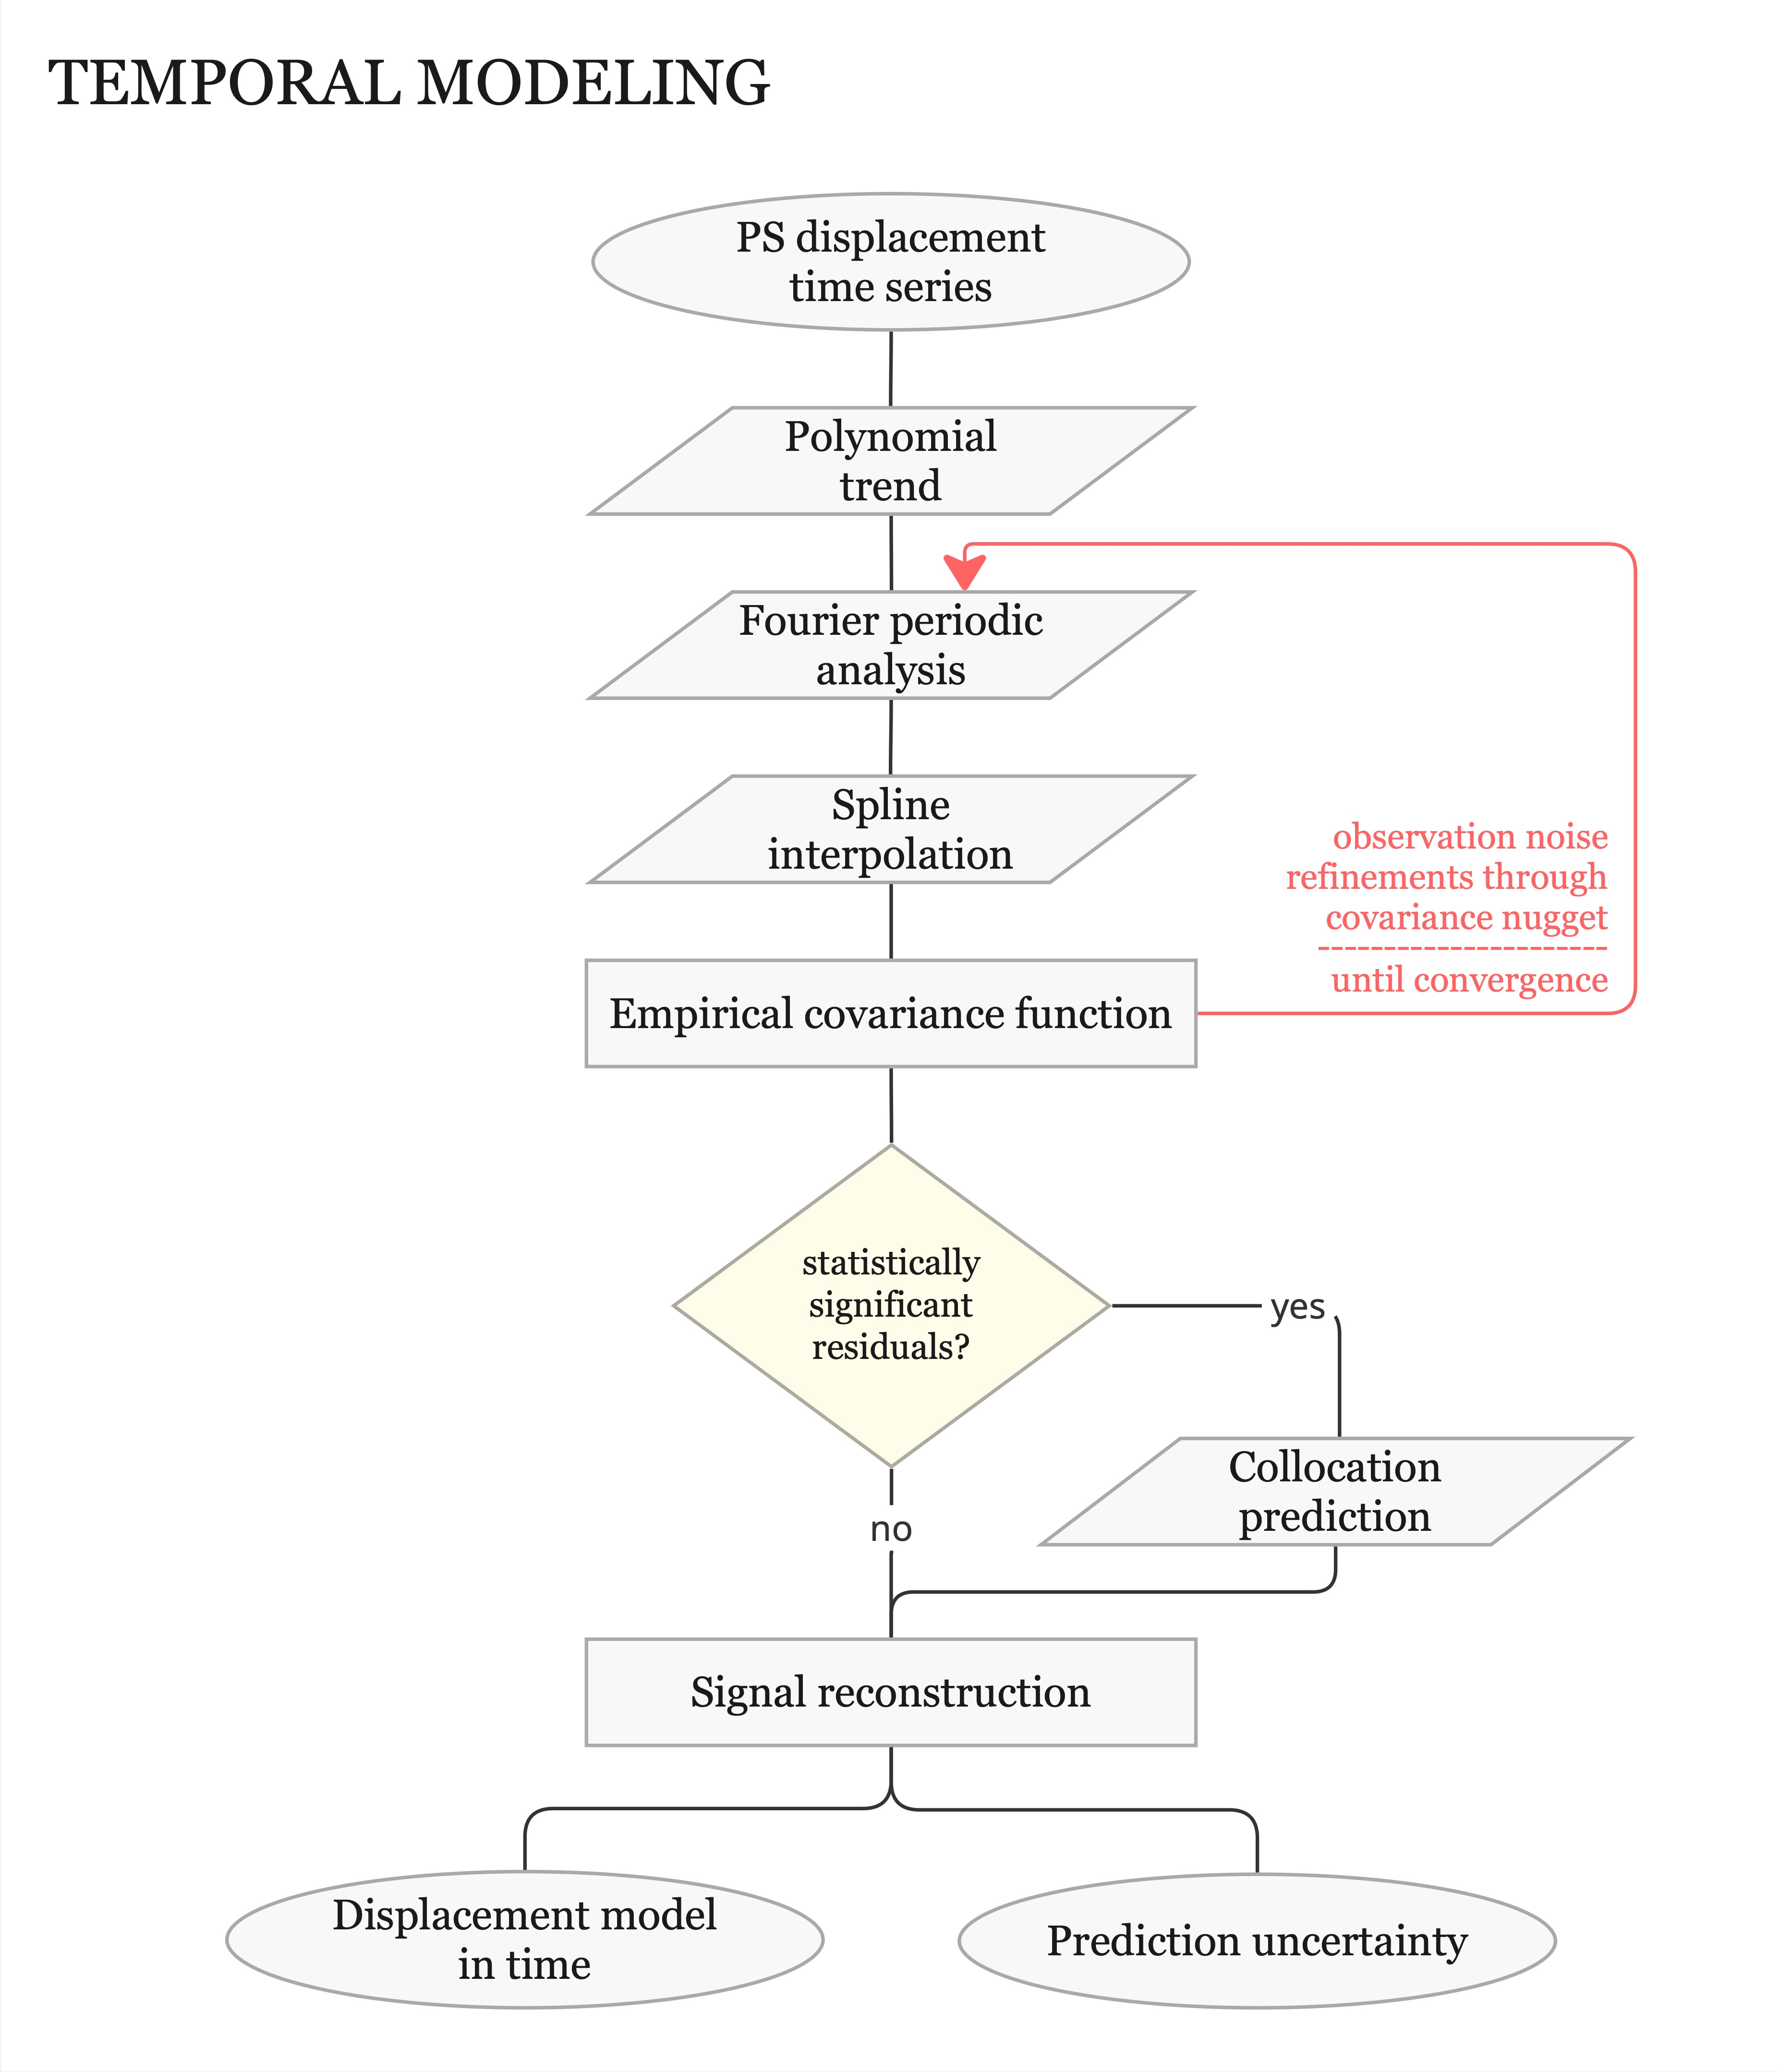
\includegraphics[width=1\textwidth]{images/G_temporal_modelling.jpg}
    \caption{Schematic representation of the temporal modeling workflow. Each PS time series is decomposed into deterministic, periodic, local, and stochastic components.}
    \label{fig:temporal_workflow}
\end{figure}

\begin{enumerate}
    \item \textbf{Deterministic trend estimation:} isolates the long-term linear or polynomial deformation component.
    \item \textbf{Periodic/seasonal analysis:} identifies and isolates cyclic thermal or seasonal oscillations.
    \item \textbf{Local modeling with splines:} captures non-linear, localized kinematic behaviors.
    \item \textbf{Empirical covariance estimation:} analyzes the residual stochastic (random) process.
    \item \textbf{Collocation:} applies filtering or prediction to obtain a smoothed, physically consistent time series.
    \item \textbf{Optional spatial visualization:} generates a quick spatial overview using Nearest Neighbor Interpolation (NNI).
\end{enumerate}

\subsubsection{Final signal reconstruction}
Because the model is built sequentially, the final reconstructed displacement estimate $\hat{d}(t)$ for any given PS is simply the sum of the isolated physical components evaluated at the target epochs:
\begin{equation}\label{eq:displ_tot}
    \hat{d}(t) = \hat{d}_{\text{trend}}(t) + \hat{d}_{\text{periodic}}(t) + \hat{d}_{\text{spline}}(t) + \hat{d}_{\text{collocation}}(t)
\end{equation}

\textbf{Understanding uncertainty:} Because each component is estimated conditionally based on the previously removed signals, you cannot simply add their individual standard deviations together. Therefore, the total uncertainty of the fully reconstructed time series $\sigma_{\hat{d}}(t)$ is represented solely by the point-wise prediction variance of the final modeled residuals.

Depending on whether the stochastic signal is physically significant enough to trigger collocation, the final reported uncertainty is defined as:
\begin{equation}
{\sigma}^2_{\hat{d}}(t) \approx
\begin{cases}
    {\sigma}^2_{\hat{d}_{\text{spline}}}(t) & \begin{array}{@{}l@{}} \text{if stochastic signal is negligible} \\ \text{(collocation skipped)} \end{array} \\
    {\sigma}^2_{\hat{d}_{\text{collocation}}}(t) & \text{otherwise}
\end{cases}
\end{equation}


\subsection{Spatio-temporal stochastic}\label{sec:1D_stc}
The stochastic approach evaluates the behavior of all PS points simultaneously. This allows the software to rigorously filter out spatially uncorrelated noise (e.g., phase unwrapping errors) and statistically interpolate data across areas lacking radar targets.

The complete procedural sequence for this stochastic spatio-temporal modeling is schematized in Figure~\ref{fig:diag_stoch}. This is valid for both 1D and 2D geometries.

\begin{figure}[H]
    \centering
    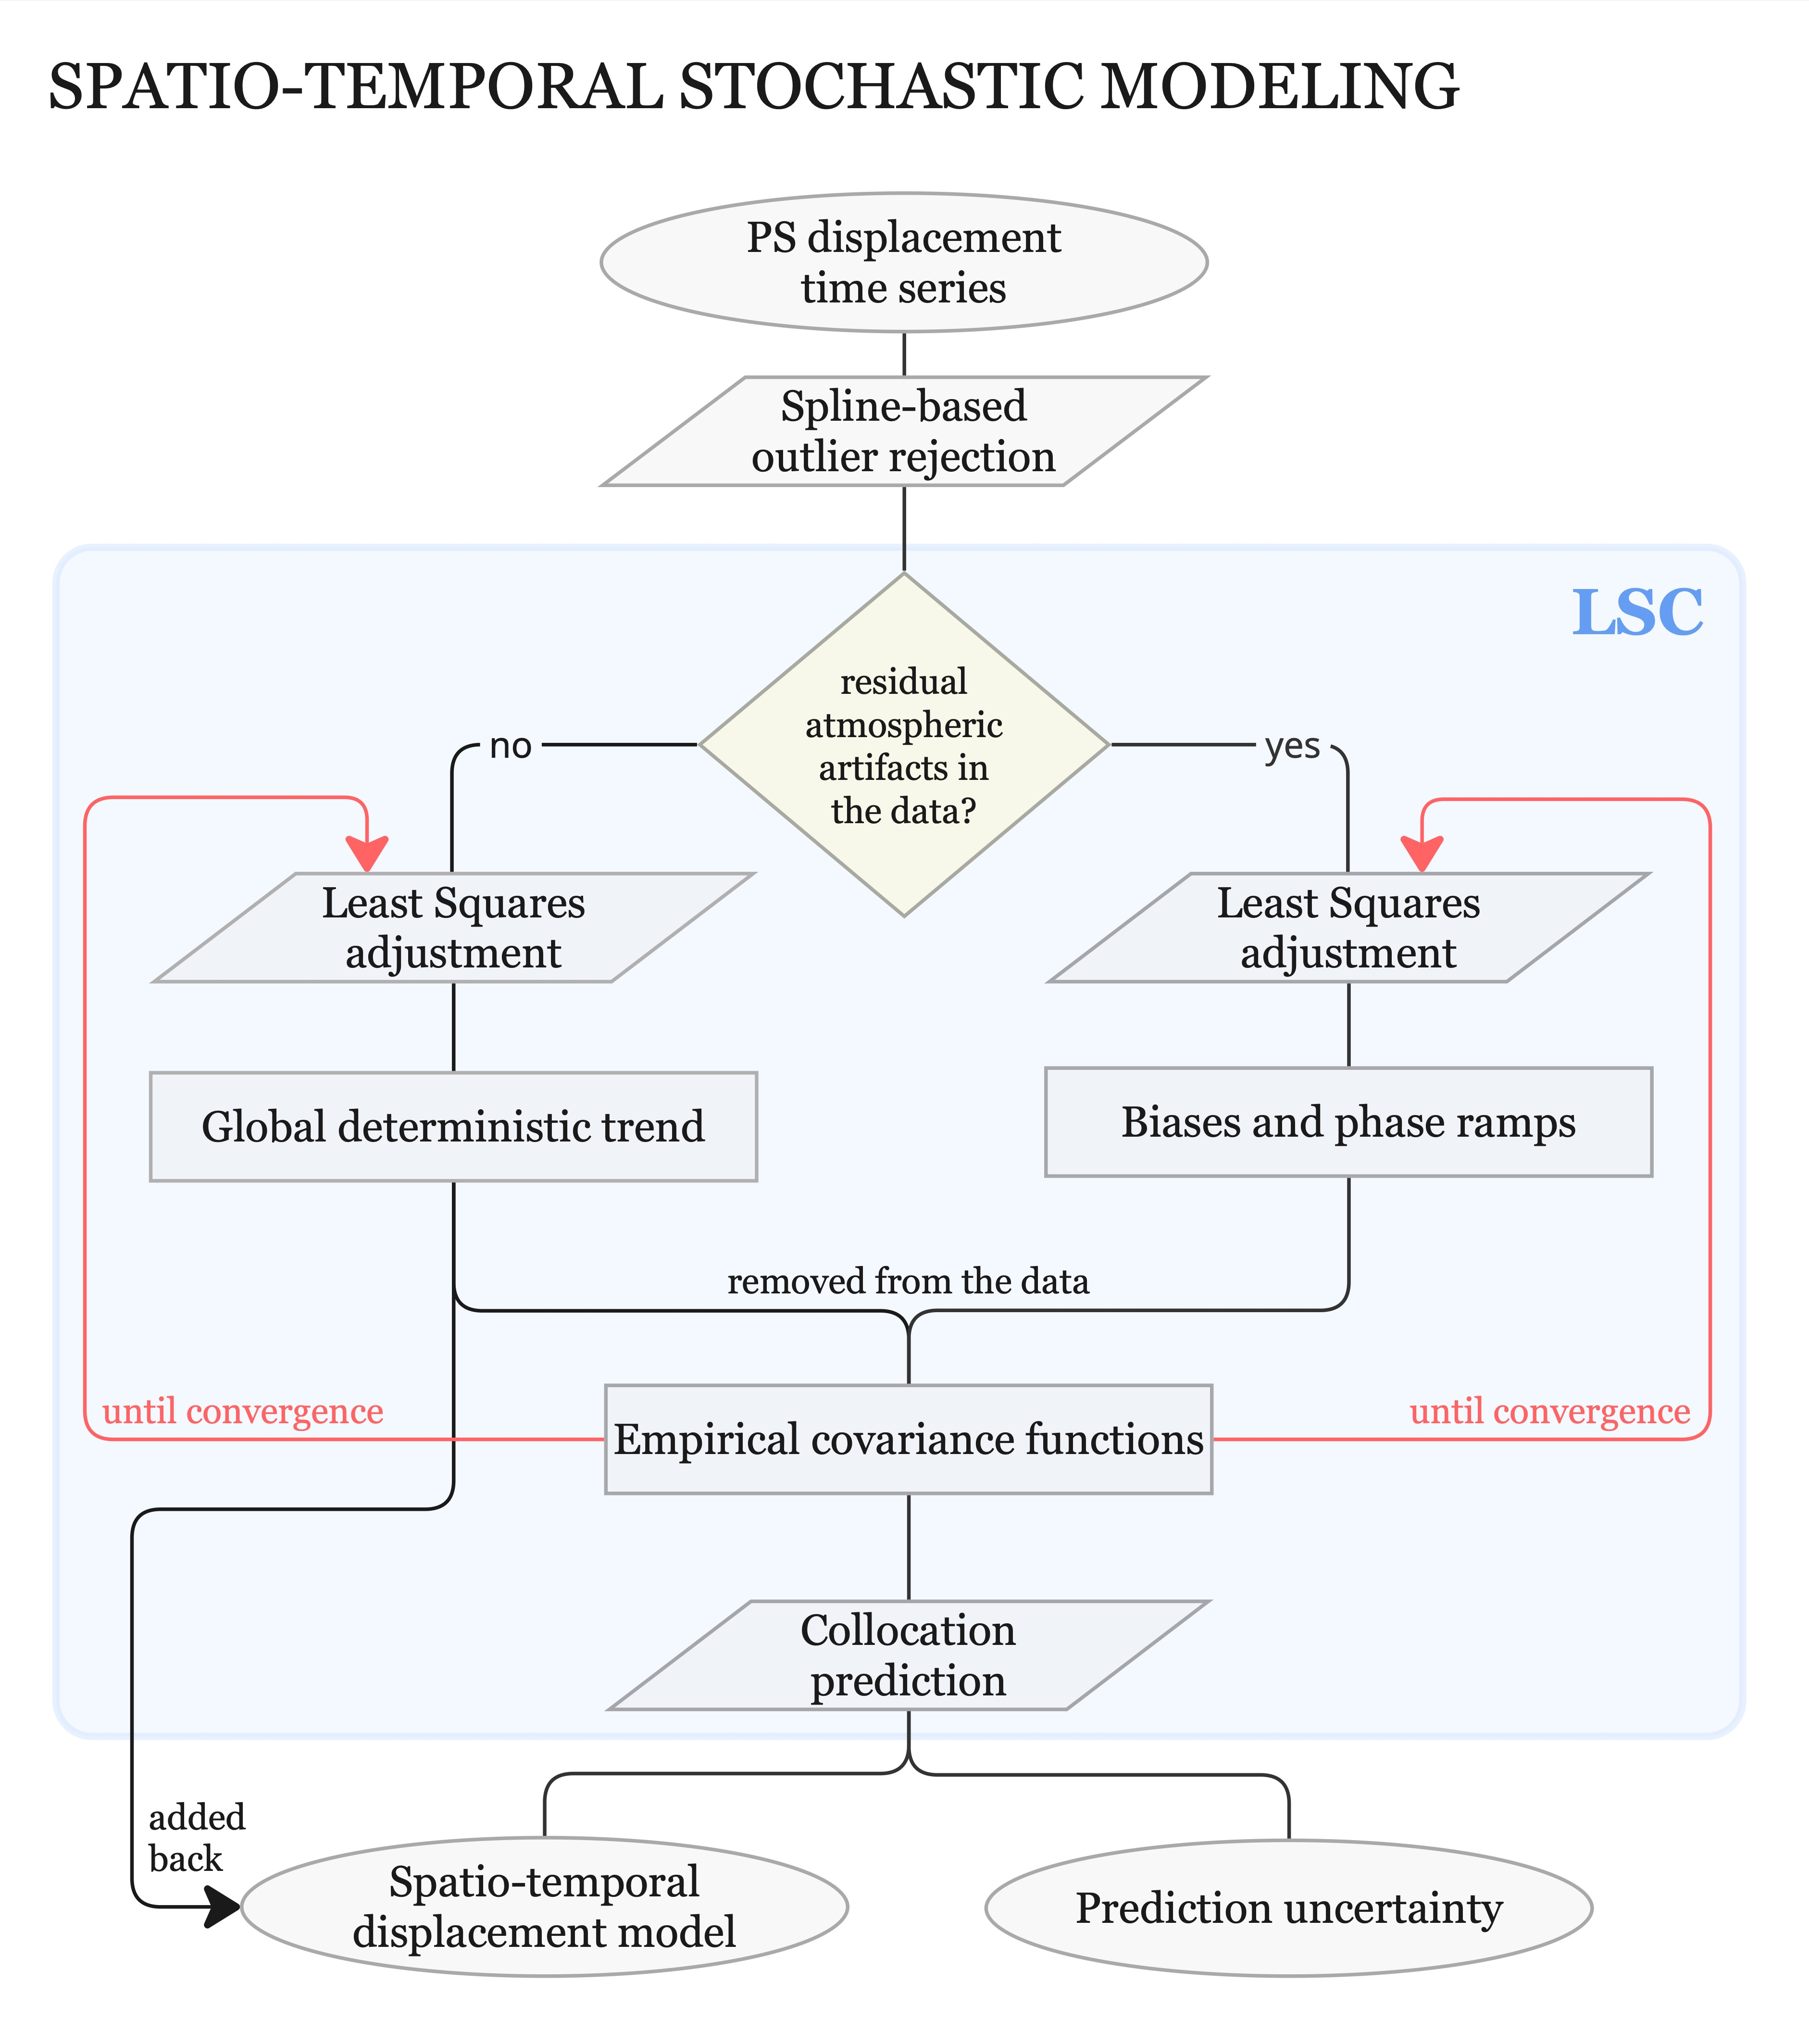
\includegraphics[width=1\textwidth]{images/G_ST_stochastic.jpg}
    \caption{Schematic representation of the stochastic spatio-temporal modeling workflow, progressing from raw PS observations through outlier rejection, empirical covariance fitting, and LSC.}
    \label{fig:diag_stoch}
\end{figure}

To facilitate the interpretation of this massive, multi-dimensional dataset, the software automatically generates dynamic and static visualizations as the final step of the processing workflow:
\begin{description}
    \item[Dynamic time-lapse (GIF):] a continuous animation is produced displaying the reconstructed displacement field superimposed on a satellite basemap. This allows users to visually track the progression of deformation phenomena throughout the entire monitoring period.
    \item[Static spatio-temporal maps:] \textit{only for 1D spatial geometry} to fit both the spatial and temporal dimensions into a single plot, the software generates 2D raster maps where the X-axis represents the curvilinear centerline coordinate ($\ell$), the Y-axis represents time ($t$), and the color scale represents the continuous displacement magnitude. An identical accompanying map is generated for the estimation uncertainty ($\boldsymbol{\sigma}_{\hat{d}}$), providing a quantitative assessment of the model reliability across space and time.
\end{description}


\subsubsection{1D spatial domain}
The workflow is configured through the 1D stochastic controls, providing access to the underlying statistical estimators without manual code modifications.

Through this interface, you govern the specific estimators used in the Least Squares Collocation framework. Key configurable parameters include:
\begin{itemize}
    \item \textbf{Centerline and time resolution:} defines the uniform spatial ($\Delta \ell^\text{out}$) and temporal ($\Delta t^\text{out}$) step sizes for the target prediction grid. This dictates the resolution of your final continuous displacement model.
    \item \textbf{Minimum period for splines fitting:} establishes the maximum flexibility of the spline curves used during the preliminary temporal outlier rejection step, preventing the algorithm from overfitting short-term noise.
    \item \textbf{Approach for LSC (Signal vs. Noise separation):} dictates how large-scale atmospheric delays and orbital errors are handled. You can choose to absorb them into the noise model, or assume clean data and fit a low-degree deterministic polynomial prior to collocation.
    \item \textbf{Atmospheric residual errors:} if present, specifies whether these errors are treated as purely time-variable biases (suitable for small AOI) or as spatio-temporal trends (required for large AOI).
    \item \textbf{Global polynomial:} defines the maximum permissible degree for the global deterministic trend fitted across the entire infrastructure axis (if assuming clean data).
    \item \textbf{Steps to average the empirical covariance:} controls the lag-binning resolution used to compute the empirical covariance point clouds. This can be determined automatically based on data density or set manually.
    \item \textbf{Covariance model:} selects the continuous mathematical function used to fit the empirical covariance data. This generates the positive-definite matrix strictly required for the final stochastic prediction.
\end{itemize}

To construct a continuous spatio-temporal deformation model along a linear infrastructure, the irregularly scattered PS observations must first be orthogonally projected onto the centerline of the element. Their spatial position is subsequently described purely by a 1D curvilinear coordinate ($\ell$), originating at the beginning of the selected segment.

\begin{quote}
    \textcolor{orange}{\textbf{WARNING:}} \textcolor{gray}{If portions of the infrastructure lack PS points (e.g., highway tunnels, which are undetectable by SAR), these sections are treated mathematically as data gaps. Because this model generates a continuous field, displacement values within these gaps are the result of pure statistical extrapolation. Always interpret extrapolated values in large data gaps with caution.}
\end{quote}

Once projected, the available displacement time series undergo a multi-step processing workflow to filter noise, remove artifacts, and prepare the data for geostatistical interpolation.


\subsubsection{2D spatial domain}
When the AOI represents a spatially distributed target---such as an urban center, a volcanic caldera, or a subsidence bowl---constraining the deformation to a 1D centerline is physically inappropriate. To address this, PHASE extends the stochastic modeling framework into a full 2D planar geometry.

The algorithmic pipeline for the 2D case is a direct extension of the 1D workflow. The mathematical estimators, outlier rejection testing, and iterative covariance updates remain fundamentally identical. The core differences lie strictly in the geometric definition of the spatial domain (incorporating the assumption of spatial homogeneity and isotropy) and the 2D expansion of the deterministic trend models.

If this approach is selected, the 2D stochastic controls become available. The parameters largely mirror the 1D configuration, with a planar spatial-resolution definition.

In the 2D domain, the \textbf{spatial and time resolution} parameter defines a uniform grid spacing applied equally to both the Easting ($x$) and Northing ($y$) coordinates, rather than a single curvilinear distance.

\begin{quote}
    \textcolor{orange}{\textbf{WARNING:}} \textcolor{gray}{Similar to the 1D case, displacement values generated over areas lacking PS points are the result of statistical extrapolation. Because 2D extrapolation expands radially across a plane, prediction uncertainties can grow rapidly in large spatial data gaps. Always interpret the results at the edges of your PS point cloud with caution.}
\end{quote}



\subsection{Spatio-temporal deterministic (Spline-based)}\label{sec:det}
As an alternative to the stochastic framework, PHASE offers a purely deterministic modeling approach. This methodology abandons empirical covariance estimation and Least Squares Collocation entirely. Instead, the continuous spatio-temporal displacement field is modeled using multidimensional basis splines.

\textbf{Why choose this mode?} Because this approach relies purely on localized geometric fitting rather than global statistical correlation, it does not assume spatial or temporal stationarity. This makes the deterministic approach highly advantageous for modeling highly localized, sudden deformation events (e.g., an isolated structural failure or a sudden sinkhole) that might otherwise be over-smoothed by stochastic covariance averaging. Furthermore, this method is computationally lighter, making it ideal for quick assessments or for executions on machines with lower processing power.

The complete procedural sequence for this deterministic modeling is schematized in Figure~\ref{fig:diag_det}. This logical flowchart applies to both the 1D and 2D spatial domains.

\begin{figure}[H]
    \centering
    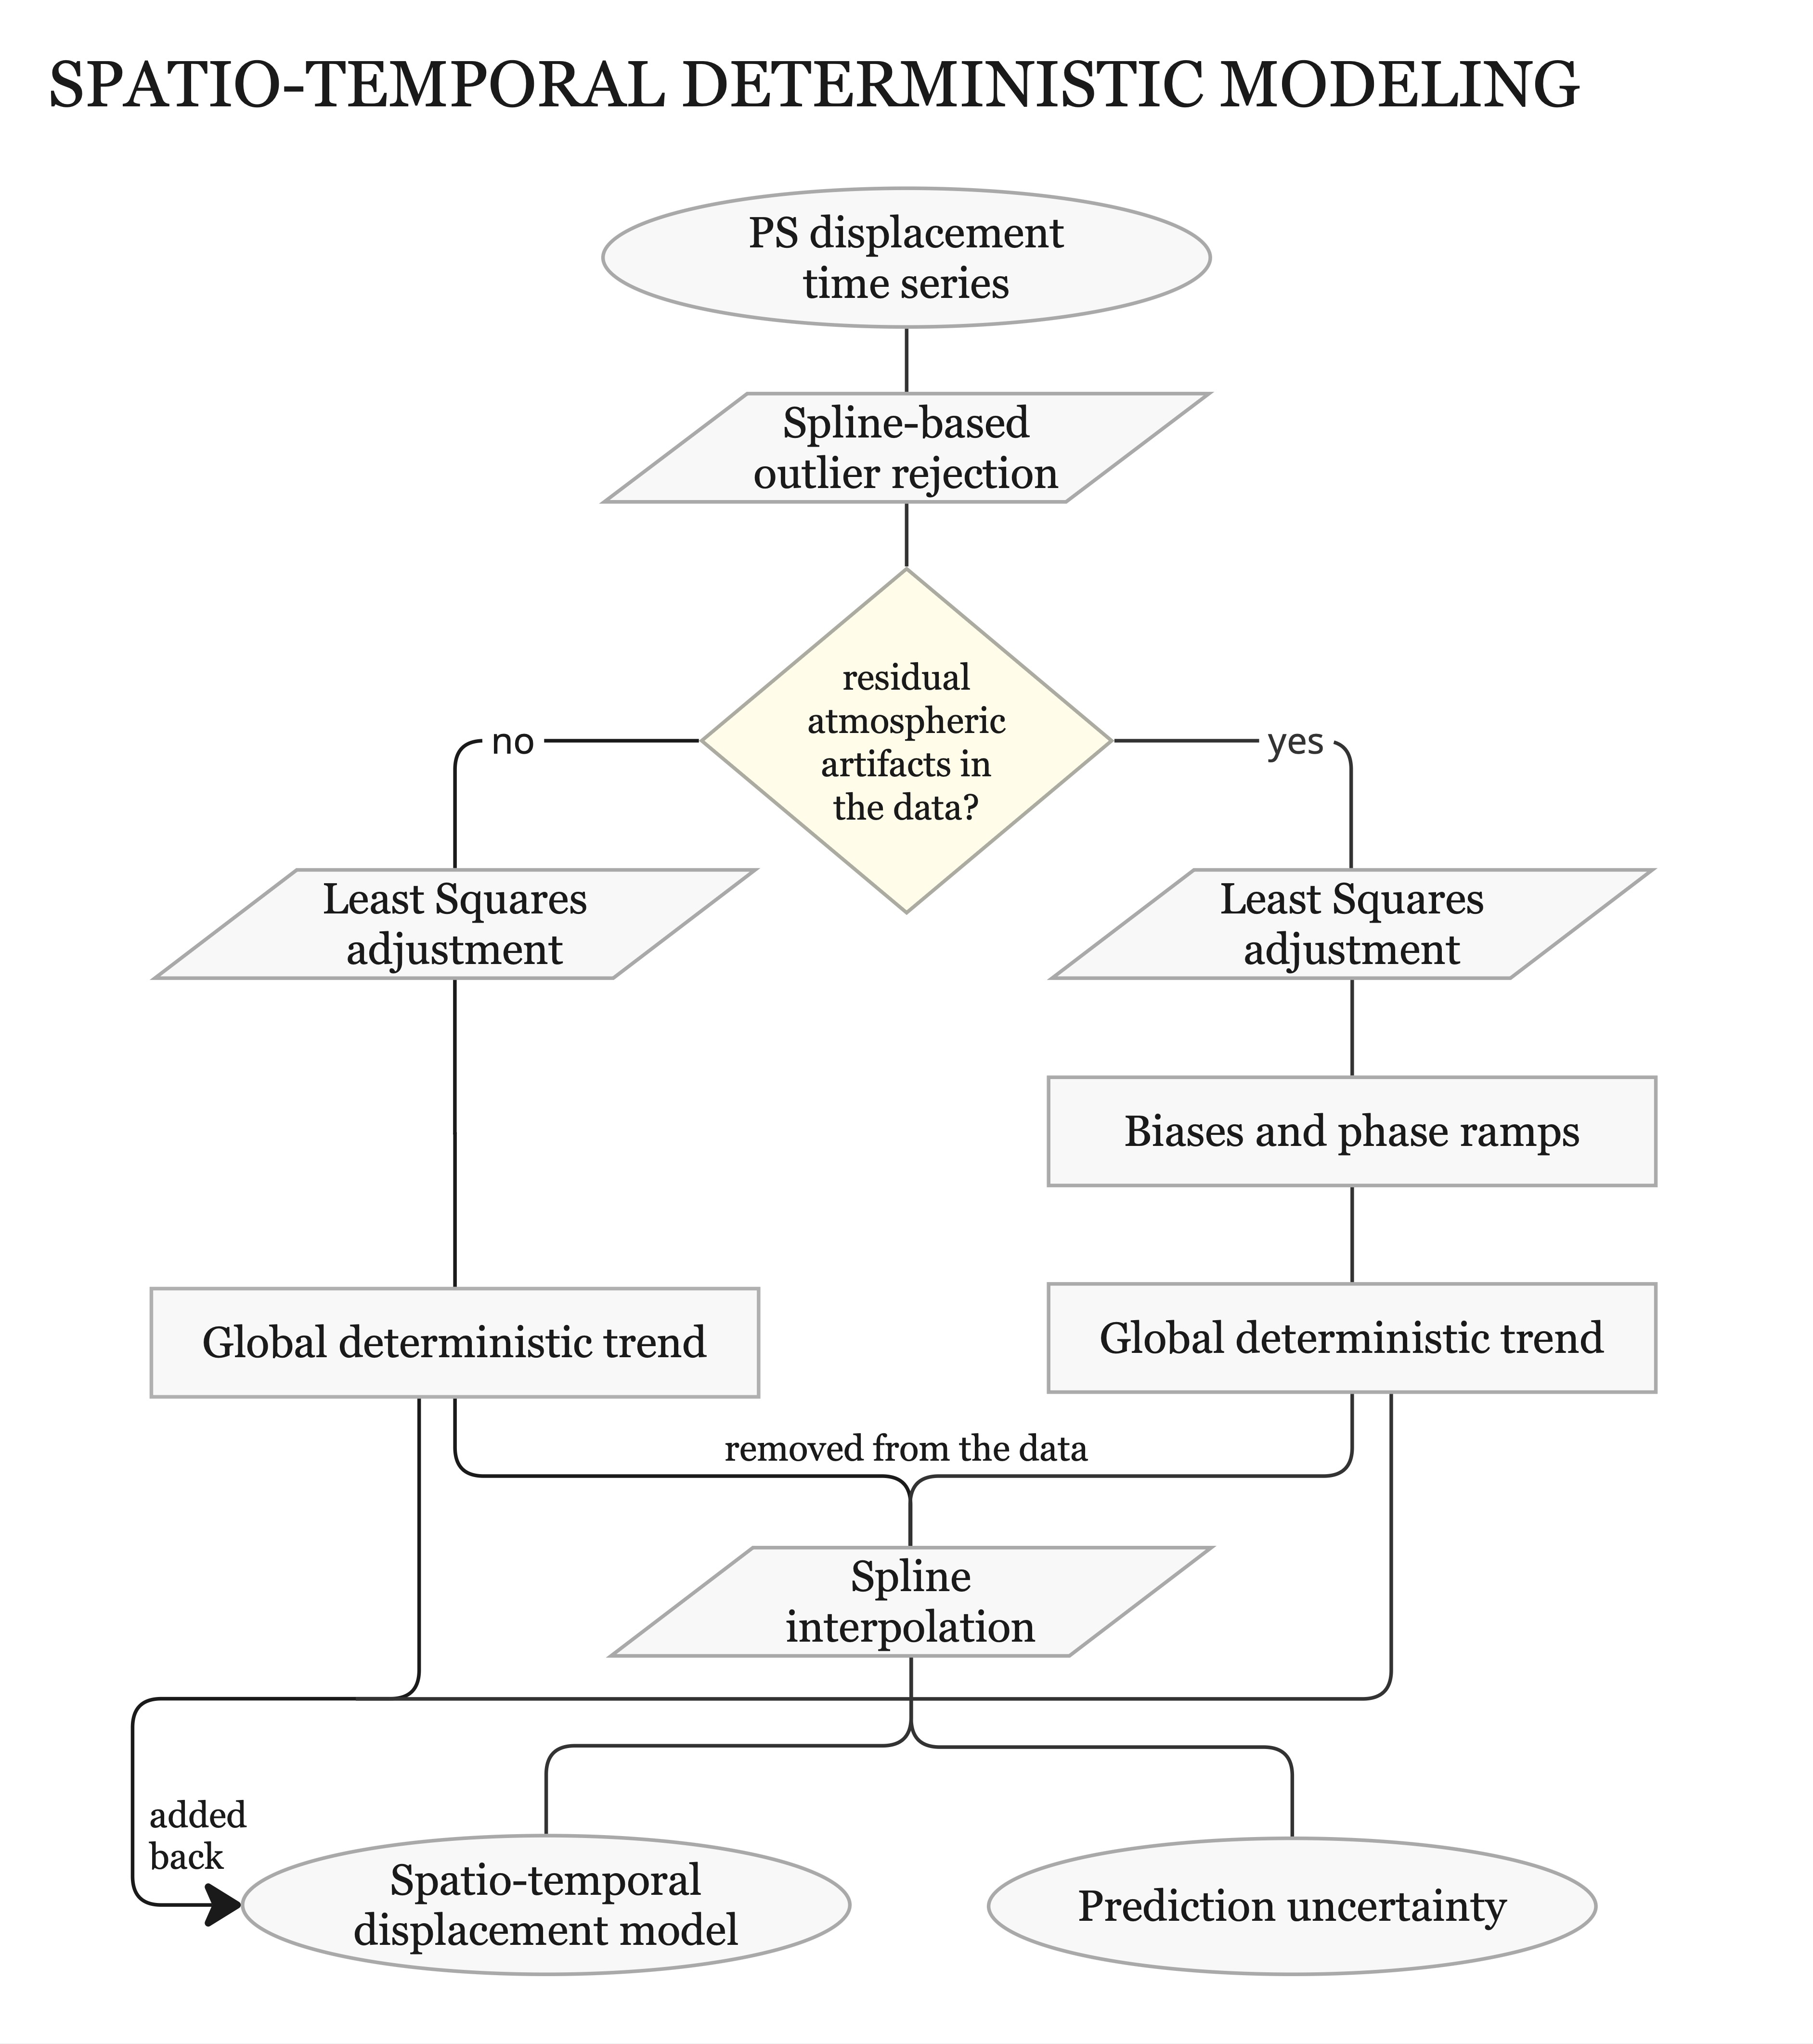
\includegraphics[width=1\textwidth]{images/G_ST_deterministic.jpg}
    \caption{Schematic representation of the deterministic spatio-temporal modeling workflow, progressing from raw PS observations through global polynomial trend removal and final multidimensional spline interpolation.}
    \label{fig:diag_det}
\end{figure}

\subsubsection{1D spatial domain}
Since the 1D infrastructure geometry involves one spatial dimension ($\ell$) and one temporal dimension ($t$), this mode fits a continuous surface using 2D bicubic splines. Configure it using the 1D deterministic controls.

Through this interface, you govern the specific estimators within the deterministic framework. Key configurable parameters include:
\begin{itemize}
    \item \textbf{Centerline and time resolution:} defines the uniform spatial ($\Delta \ell$) and temporal ($\Delta t$) step sizes for the target prediction grid upon which the final bicubic displacement surface is evaluated.
    \item \textbf{Minimum period for splines fitting:} establishes the maximum flexibility of the 1D splines used during the preliminary temporal outlier rejection step (structurally identical to the stochastic preprocessing).
    \item \textbf{Atmospheric residual errors:} if deemed present, these are estimated and removed. You can specify whether these errors are treated as purely time-variable biases (for small AOIs) or as epoch-specific spatial trends (for large AOIs).
    \item \textbf{Global trend:} defines the degree of a macroscopic spatio-temporal polynomial surface. Unlike the stochastic mode, this global surface is \textit{always} estimated and removed prior to the bicubic spline interpolation to ensure the splines only fit local, high-frequency physical deformations.
    \item \textbf{Bicubic spline optimization:} selects the strict statistical criteria (variance threshold, F-test, MDL or $\chi^2$ test) used to automatically determine the optimal number of spline knots for the final surface, preventing overfitting.
\end{itemize}

\subsubsection{2D spatial domain}
When the monitored AOI is a spatially distributed target (e.g., an urban center or a subsidence bowl), this module extends the deterministic, spline-based approach to the planar domain. It reconstructs the continuous deformation field $d(x,y,t)$ using 3D tricubic splines.

Selecting this option activates the 2D deterministic controls, which adapt the spatial resolution and optimization strategy to a planar grid.

The configuration parameters mirror those of the 1D deterministic case, adapted specifically for the expanded geometric domain. Most notably:
\begin{itemize}
    \item The \textbf{Spatial and time resolution} parameter now defines a uniform square grid spacing applied equally to both the Easting ($x$) and Northing ($y$) axes.
    \item The \textbf{Global trend} polynomial degree defines a trivariate surface instead of a bivariate one.
\end{itemize}


\subsection{Query points}
The filepath to a \texttt{.txt} file containing the coordinates (UTM or geographic) of query points can be specified in this last panel. This will trigger the interpolation module of the software to evaluate the estimated spatio-temporal model exactly at these coordinates. In the output Excel report this will result in displacement time series plots in the \textit{Interpolation} sheet.

Additionally, there is also a checkbox to export the modeled displacement time series at the observed PS positions. This can be found in the \textit{Modelled PS} sheet of the generated Excel report.


\section{Automatic report generation and data export}
To facilitate the interpretation and dissemination of the results, the software includes a fully automated workflow for report generation. Upon completion of the processing chain, the software aggregates the numerical results, the estimated statistical parameters, and the generated figures into a comprehensive Microsoft Excel spreadsheet.

The report is structured into five (or six/seven, if external interpolation and/or PS modeling is requested) specific sheets:

\subsection{General sheet}
This sheet serves as the project summary. It compiles all relevant metadata regarding the analysis, including:
\begin{itemize}
    \item \textbf{Project metadata:} date of execution, municipality, and country of the AOI (automatically geocoded from the reference PS point), and the chosen modeling strategy (e.g., 1D vs. 2D, stochastic vs. deterministic).
    \item \textbf{Input parameters:} details on the PS dataset, including the total number of scatterers, the observation period, and the unwrapping reference point coordinates. If available, the specific StaMPS processing parameters used in the upstream analysis are also reported.
    \item \textbf{Visual context:} three figures are automatically embedded: the project logo, a topographic map locating the AOI within the country, and a satellite map showing the distribution of PS points inside and outside the selected AOI (Figure~\ref{fig:sheet_general}).
\end{itemize}

\begin{figure}[H]
    \centering
    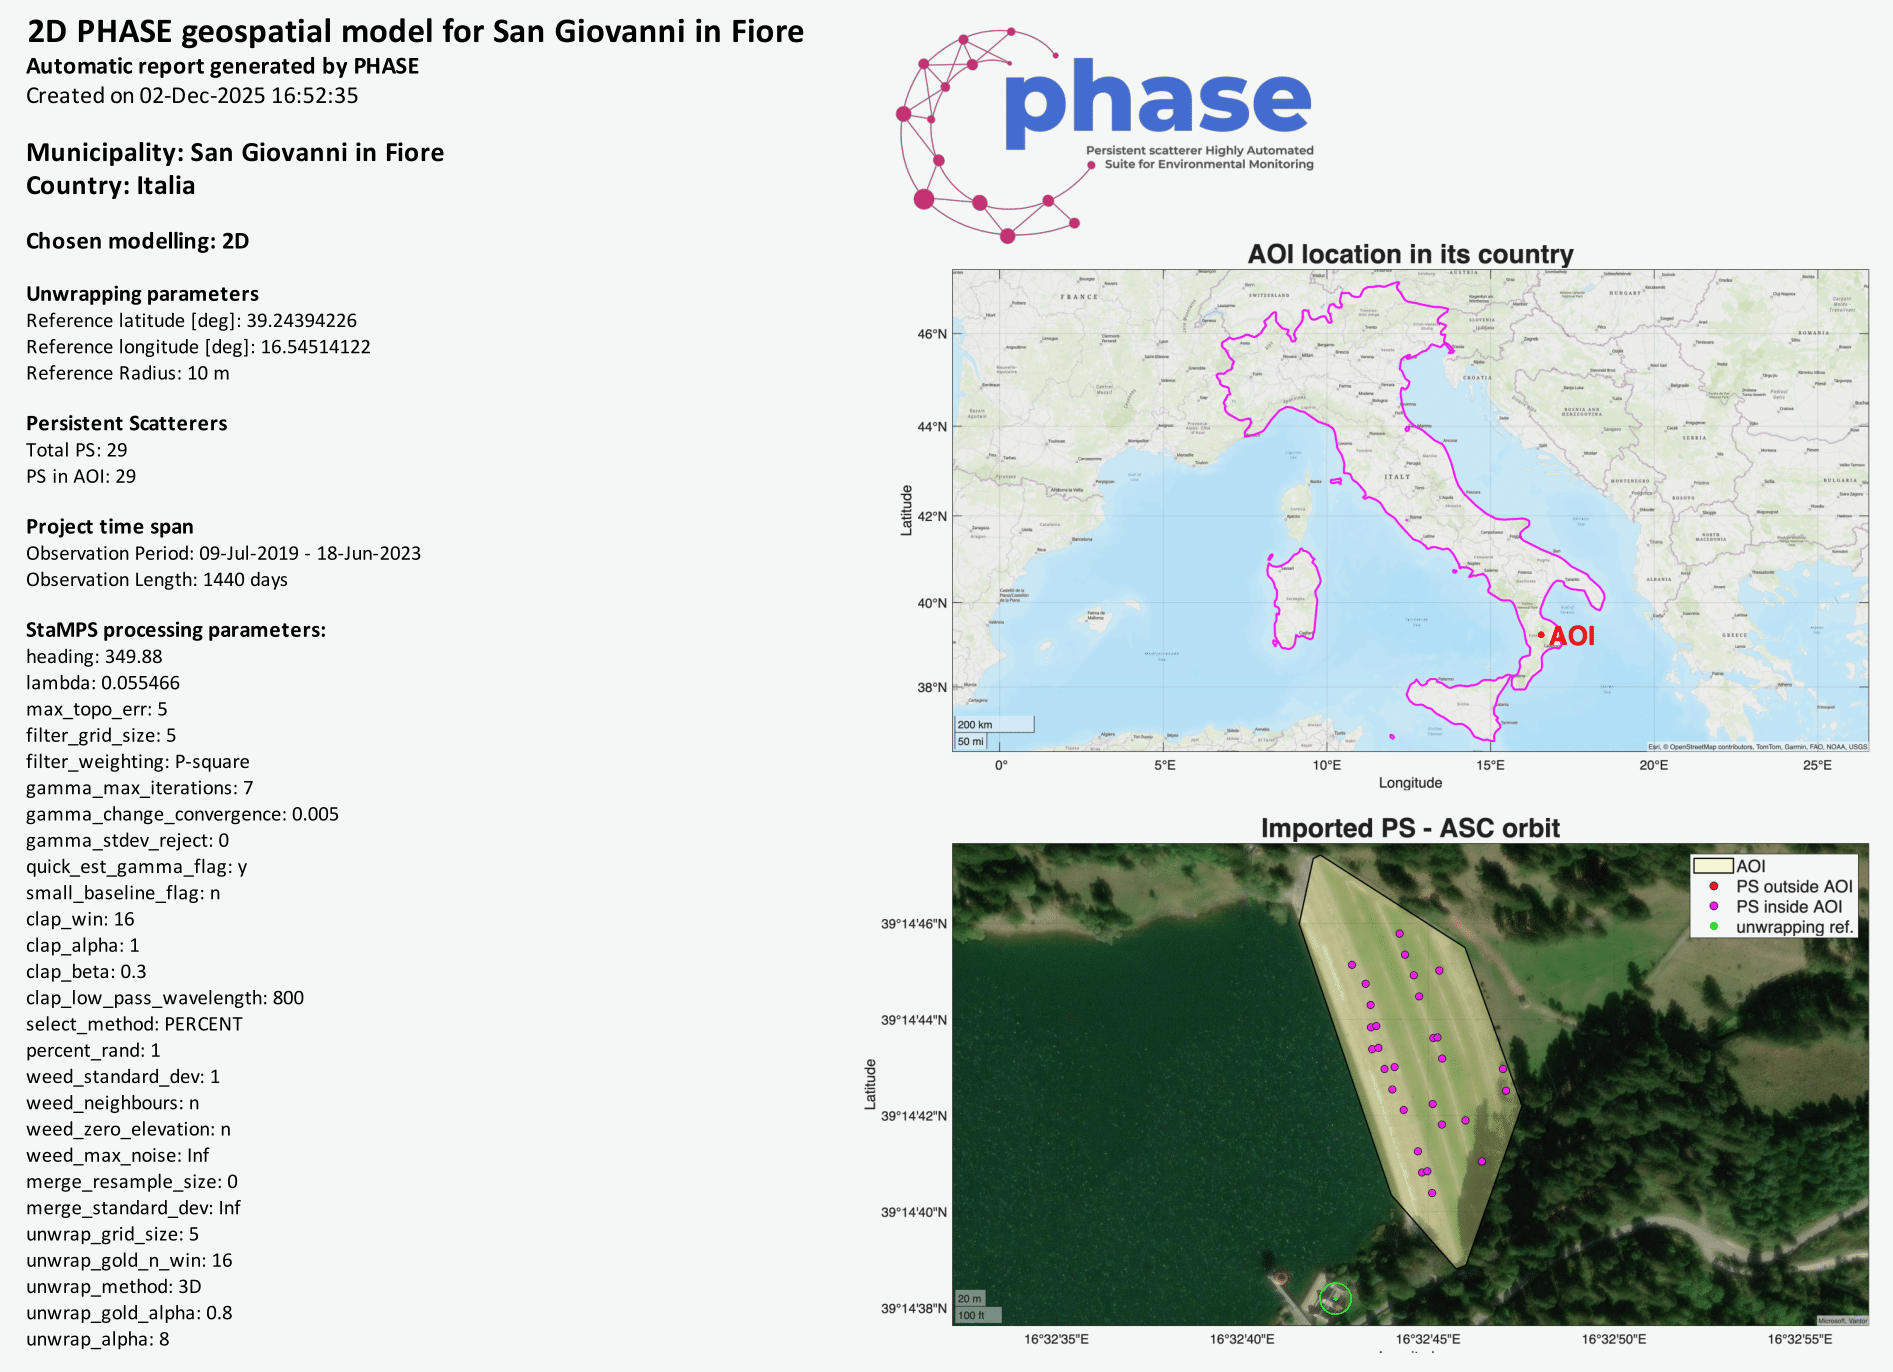
\includegraphics[width=0.9\textwidth]{images/sheet_general.png}
    \caption{Example of the \textit{General} sheet in the automatic output report, showing project metadata and context maps.}
    \label{fig:sheet_general}
\end{figure}

\subsection{Data sheets (Raw, Modeled, Uncertainty)}
Following the general overview, the core results are organized into three dedicated sheets. Each shares a similar structure: a header with summary statistics followed by the full data table, where rows represent individual PS points and columns represent observation epochs.

\begin{itemize}
    \item \textbf{Raw displacement:} contains the input PS time series after the initial detrending (subtraction of the modeled value at the first epoch). It includes a plot of the spatially averaged displacement time series over the AOI with an overlaid linear trend to identify macroscopic subsidence or uplift phenomena.
    \item \textbf{Modeled displacement:} contains the final result of the spatio-temporal modeling (stochastic or deterministic). It includes the full set of estimated displacement time series for all positions in the AOI based on the chosen spatial resolution. A map showing the average velocity (in mm/year) is embedded to provide an immediate overview of deformation rates (Figure~\ref{fig:sheet_modeled}).
    \item \textbf{Uncertainty:} mirroring the modeled displacement, this sheet reports the final-stage prediction standard deviation for every epoch and point, following the convention explained above. Its summary column and map show the arithmetic time mean of those standard deviations, not a propagated variance or an independent uncertainty estimate. This helps identify areas where predictions are less precise, for example near sparse PS coverage. In temporal-plus-NNI mode, the values at new grid locations are directly interpolated standard deviations; no interpolation covariance is propagated, so treat them as an uncertainty proxy rather than a rigorous prediction interval.
\end{itemize}

\begin{figure}[H]
    \centering
    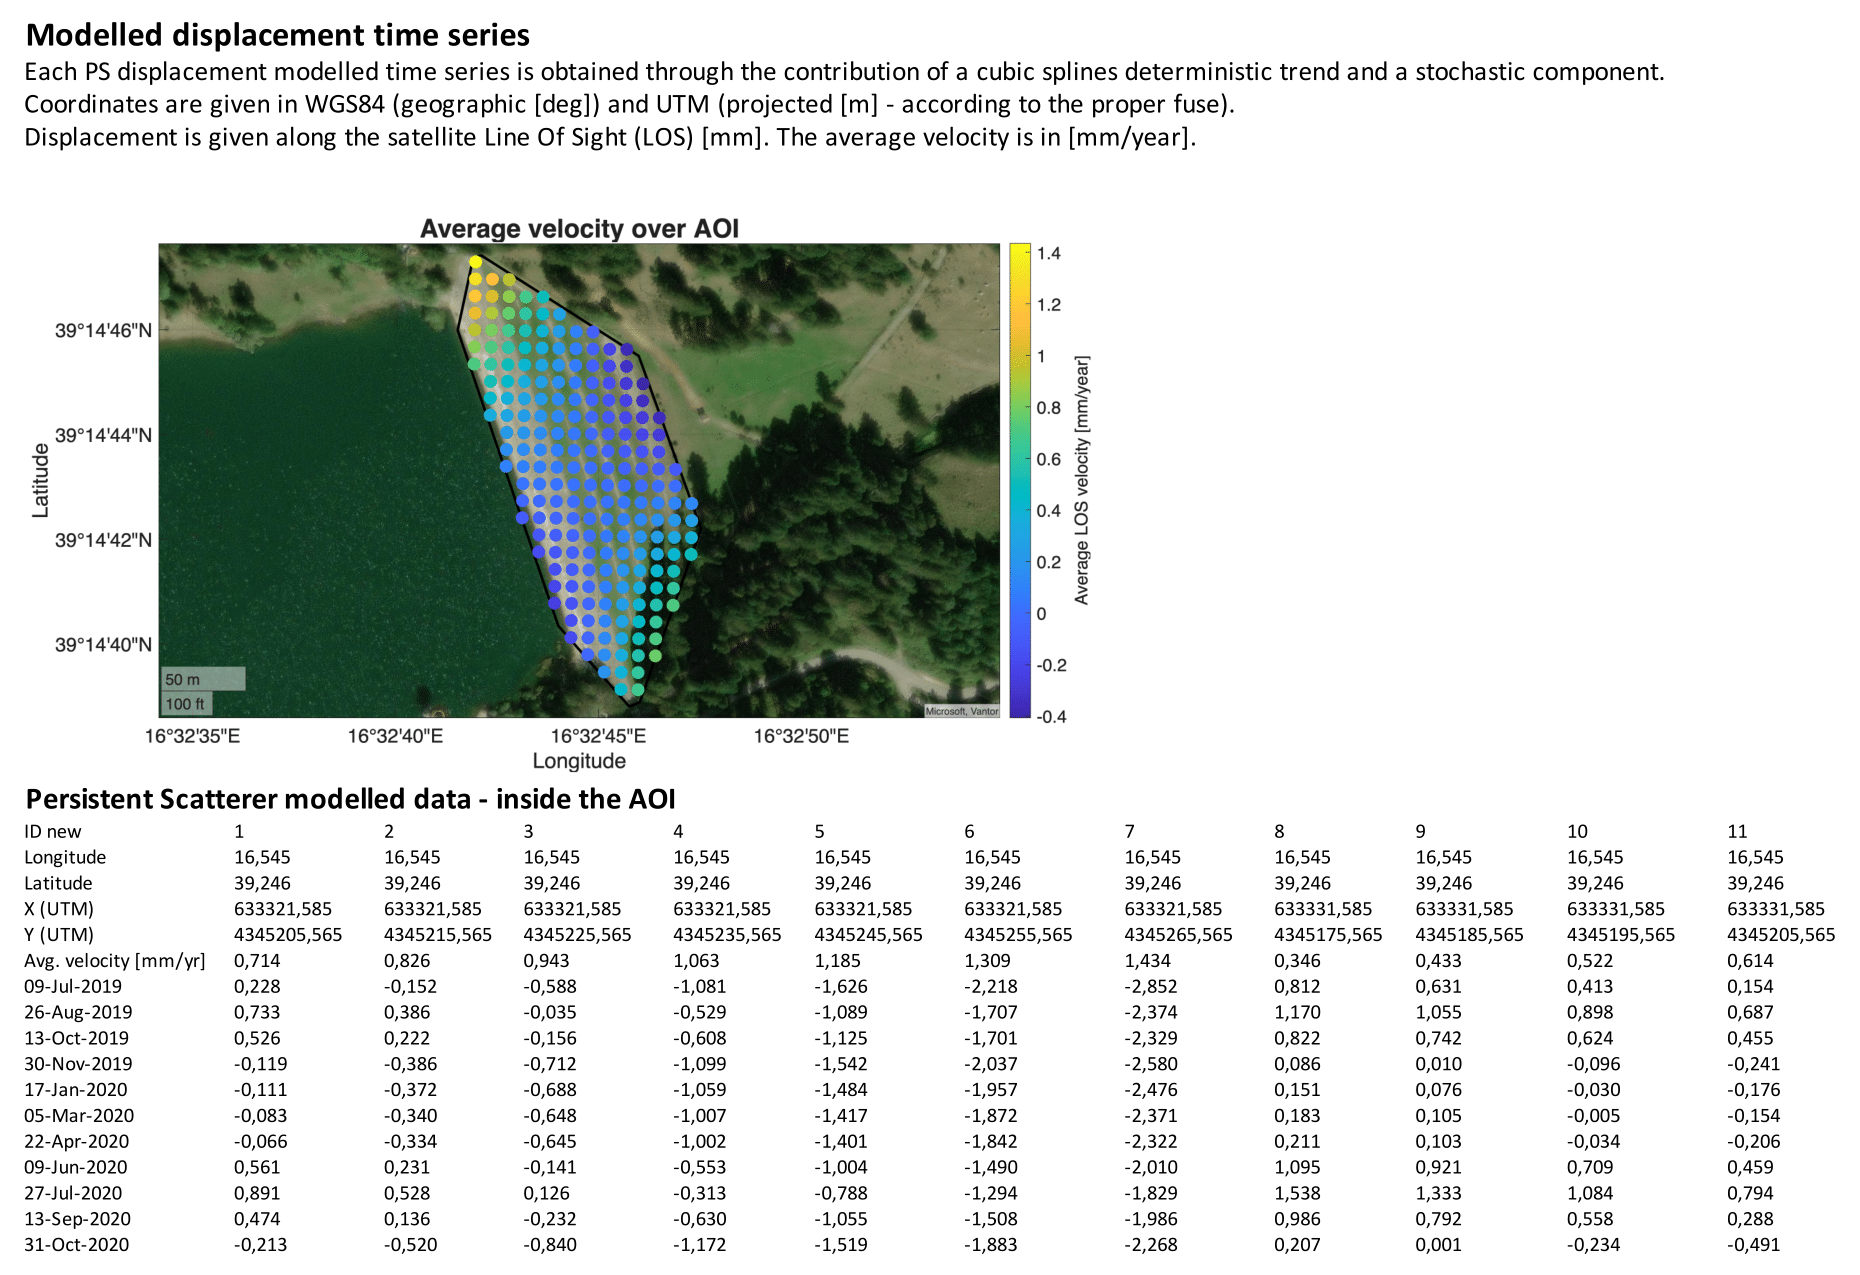
\includegraphics[width=0.9\textwidth]{images/sheet_modelled.png}
    \caption{Example of the \textit{Modeled displacement} sheet, featuring the data table and the average velocity map.}
    \label{fig:sheet_modeled}
\end{figure}

\subsection{Interpolation sheet (optional)}
If you provide a set of specific target coordinates (e.g., GNSS stations or critical infrastructure points), this sheet reports the displacement time series extracted from the continuous spatio-temporal model at those exact locations. This feature allows you to retrieve the deformation history at arbitrary points, regardless of the original PS distribution. For each target point, a specific plot showing the temporal evolution of the displacement is automatically generated and embedded.

\subsection{Modelled PS sheet (optional)}
If you flag this option, this sheet reports the displacement time series extracted from the continuous spatio-temporal model at the observed PS coordinates.

\subsection{AOI anomalies sheet (descriptive comparison)}
The \textit{AOI anomalies} sheet compares each complete \emph{modelled} LOS displacement series with the AOI median at each epoch. This highlights locations whose fitted deformation differs from the rest of the AOI without treating a noisy raw-observation residual as a deformation anomaly. For regularly spaced 1D centerlines or 2D grids, each modelled location has equal length or area weight in this comparison.

At each epoch $t$, the reference is the spatial median $m(t)$ of modelled displacement $\hat d_i(t)$. The robust AOI scale is $1.4826\,\operatorname{median}_i|\hat d_i(t)-m(t)|$, bounded below by the spatial median of the reported prediction standard deviations. The output lists the maximum absolute deviation in millimetres, the maximum deviation divided by this scale, and the fraction of epochs with normalized contrast at least three. A \textit{transient} or \textit{persistent} label requires two consecutive modelled epochs above that descriptive threshold; persistence of at least 20\% of epochs yields \textit{persistent}. Average velocity remains available as context, but does not determine the label. These scores are relative to the selected AOI and are neither hazard probabilities nor formal significance tests. Changing the AOI can change the reference and the labels.

\subsection{GIS and data export}
Finally, in addition to the Excel report, the software automatically exports the results in GIS-compatible formats to facilitate integration with other geospatial workflows:
\begin{itemize}
    \item \textbf{ESRI Shapefile (\texttt{.shp}):} a vector point file containing all points with their attributes (ID, coordinates, average velocity, time-mean prediction standard deviation and descriptive AOI-anomaly class/contrast) and the full displacement time series as additional columns (one for each date). A \texttt{.prj} file defines the output coordinates as WGS84.
    \item \textbf{MATLAB data (\texttt{.mat}):} a structure array containing the same data for advanced post-processing directly in MATLAB.
    \item \textbf{GeoTIFF (\texttt{.tif}):} a multi-band GeoTIFF file containing the georeferenced displacement and uncertainty maps at each query epoch.
\end{itemize}

These outputs summarize the PSI post-processing, providing ready-to-use data that can be immediately ingested into monitoring algorithms, decision-making chains, and research activities.



% --- Appendix Starts Here ---
\part{Appendix}
\appendix
\chapter{Preprocessing with External DEM}

When employing an external Digital Elevation Model (DEM) in the \texttt{snap2stamps} procedure, it is mandatory that the file is in the correct format.

\section{File Requirements}
\begin{itemize}
    \item \textbf{File Type:} \texttt{.tif} (GeoTIFF)
    \item \textbf{Reference System:} WGS 84 - EPSG:4326
\end{itemize}

\section{Preparation Procedure (QGIS)}
To prepare the DEM, you can use QGIS to reproject the input DEM according to the source data requirements.

\begin{enumerate}
    \item Open QGIS and load your DEM.
    \item Open the \textbf{Warp (Reproject)} tool.
    \item Set the \textbf{Target CRS} to \texttt{EPSG:4326}.
    \item \textbf{Important:} Define \texttt{0} as the \enquote{Nodata value} in the reproject toolbox settings. \textit{(Note: While 0 is not a standard NoData value in general GIS practices, it is strictly required here because the value 0.0 is hardcoded into the snap2stamps XML graph parameters. Using any other value will cause SNAP to crash during processing).}
\end{enumerate}

\begin{figure}[H]
    \centering
    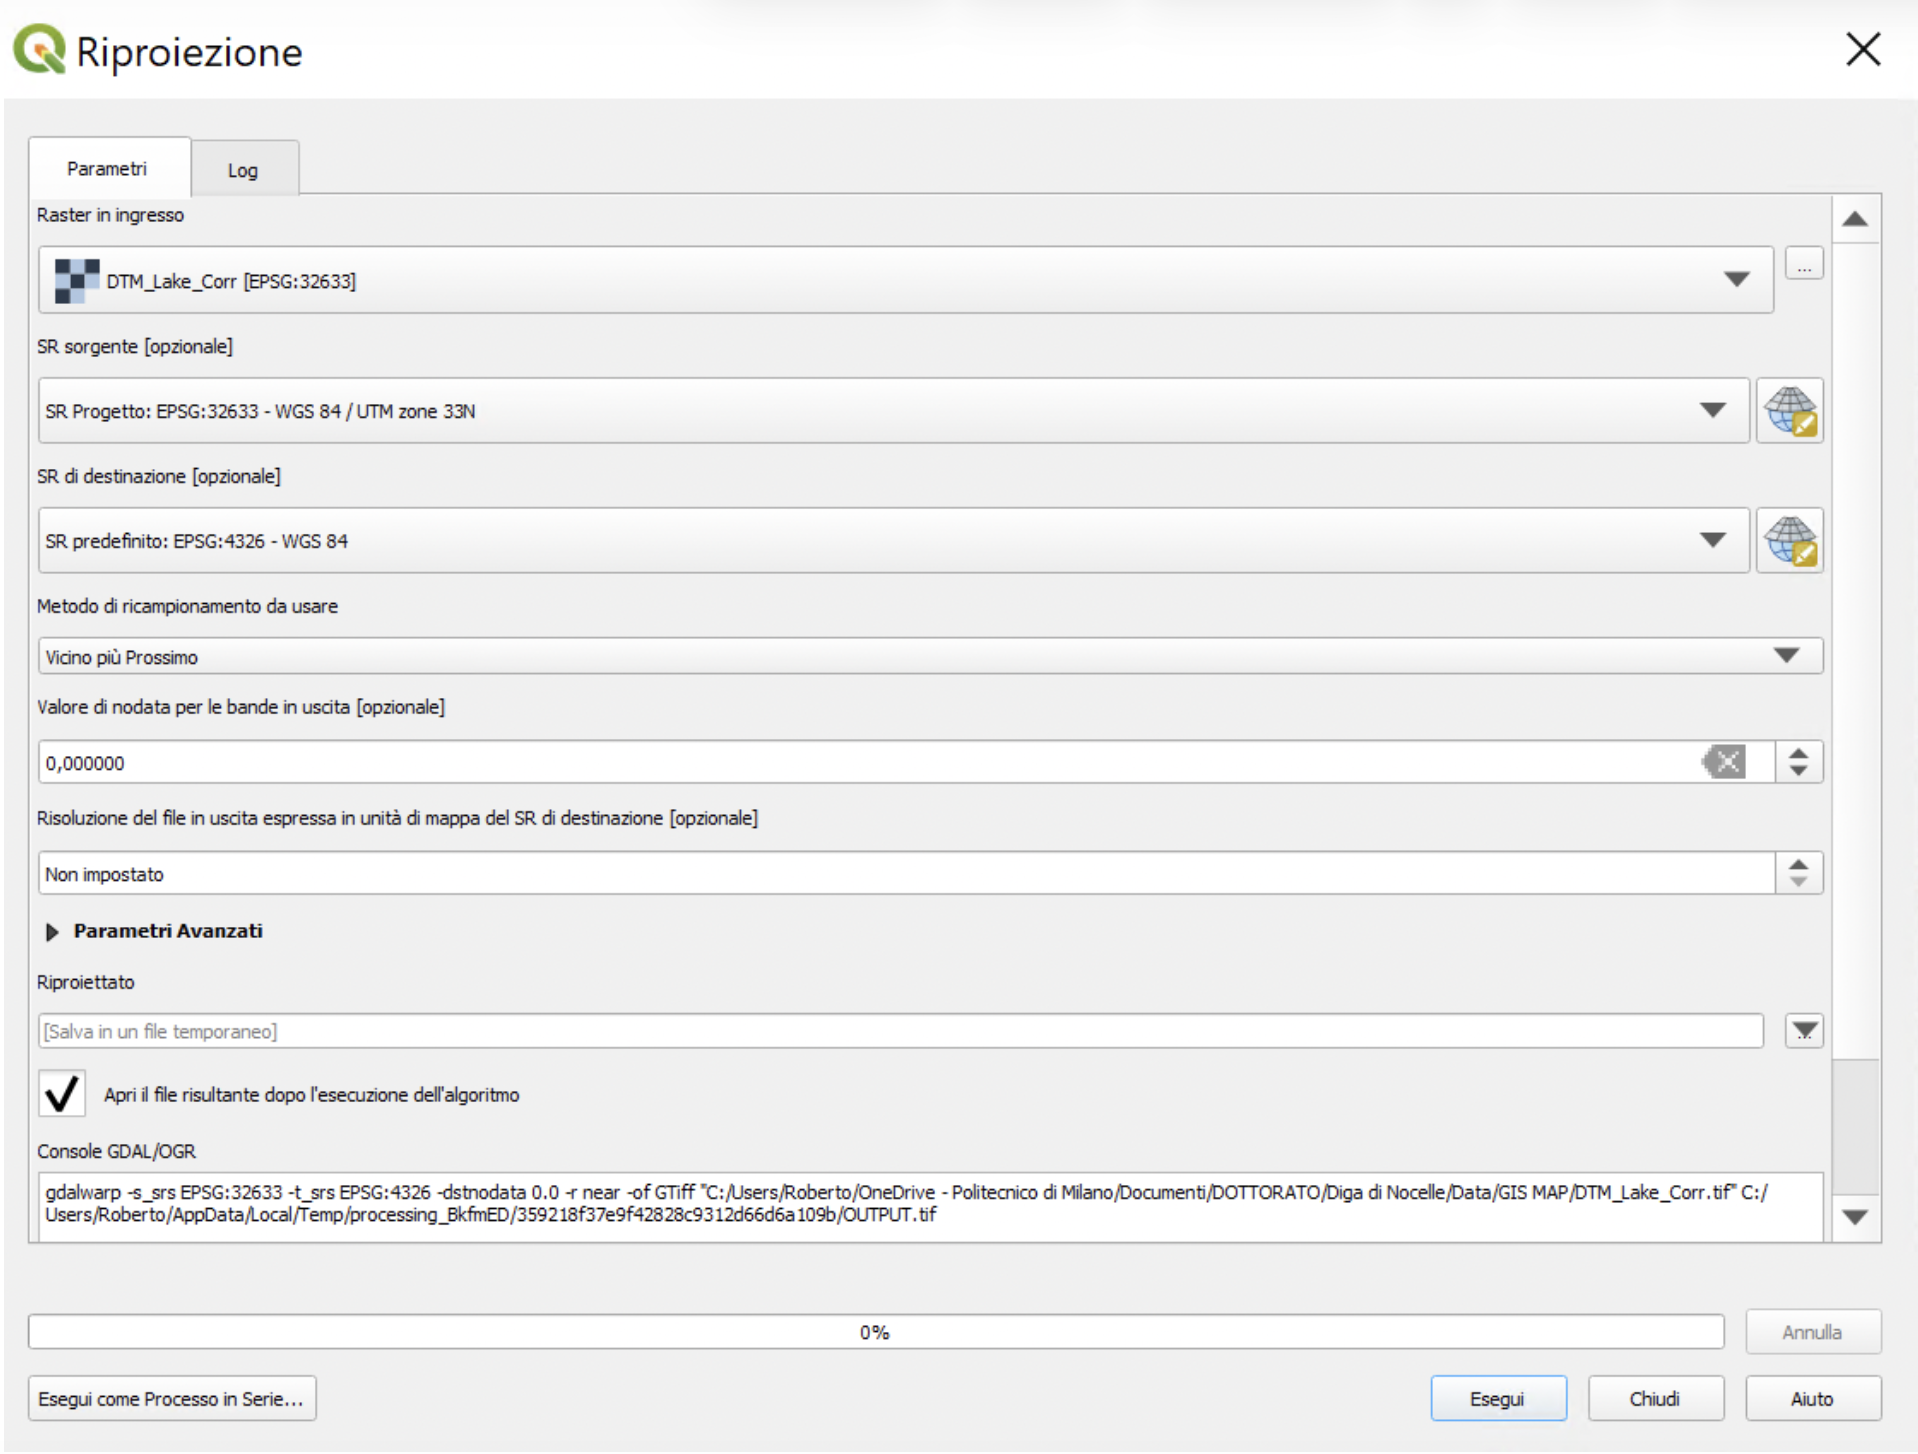
\includegraphics[width=0.8\textwidth]{images/qgis_reproject.png}
    \caption{QGIS Reprojection Settings.}
\end{figure}

\begin{quote}
    \textcolor{cyan}{\textbf{SUGGESTION:}} For successful processing, it is recommended that the External DEM covers an area that is approximately \textbf{10\% larger} than the Area of Interest (AOI) set for the subset of the SAR images.
\end{quote}

\bibliographystyle{plainnat}
\nobibliography{references} % This matches the filename 'references.bib'

\end{document}
